%*******************************************************************************
%*********************************** Chapter DUNE ******************************
%*******************************************************************************
\chapter{The Deep Underground Neutrino Experiment}  %Title of chapter

\graphicspath{{DUNE/Figs/PDF/}{DUNE/Figs/Raster/}{DUNE/Figs/Vector}}

%%% LArSoft section
\nomenclature[a-tick]{tick}{Unit of time equal to 500 ns}
\nomenclature[z-CRC]{CRC}{Cosmic Ray Counter}
\nomenclature[z-SiPM]{ADC}{Analogue to Digital Converter}
\nomenclature[z-SiPM]{SiPM}{Silicon Photo Multiplier}

%%% The main DUNE section
\nomenclature[z-FD]{FD}{Far Detector}
\nomenclature[z-FD]{FD}{Far Detector}
\nomenclature[z-DUNE]{DUNE}{Deep Underground Neutrino Experiment}
\nomenclature[z-LBNF]{LBNF}{Long Baseline Neutrino Facility}
\nomenclature[z-LBNF]{LBNE}{Long Baseline Neutrino Experiment}
\nomenclature[z-LBNF]{LBNO}{Long Baseline Neutrino Observatory}
\nomenclature[z-SURF]{SURF}{Sanford Underground Research Facility}
\nomenclature[z-PIP-II]{PIP-II}{Proton Improvement Plan II}



The Deep Underground Neutrino Experiment (DUNE) is a next-generation nuetrino experiment, which came about through the recommendations of the P5 report in 2014~\citep{P5Doc}. It was largely formed by the merger of two competing next-generation neutrino experiments, the Long Baseline Neutruno Experiment (LBNE)~\citep{LBNE_CDR1, LBNE_CDR2, LBNE_CDR3, LBNE_CDR4, LBNE_CDR5, LBNE_CDR6} a US-based experiment, and the Long Baseline Neutrino Observatory (LBNO)~\citep{LBNO_EOI} a European-based experiment. \\

The DUNE Far Detector (FD) will consist of four modules, each of which is a 10 kt Liquid Argon (LAr) Time Projection Chamber (TPC) (LArTPC). The four FD modules will be 4850 ft below ground, at the Sanford Underground Research Facility (SURF). This detector location is 1300 km away Fermilab, from which DUNE will recieve a neutrino beam with a beam power of 1.2 MW, this will increasing to 2.4 MW through upgrades during the lifetime of the experiment. Located at Fermilab will also be a high resolution and high precision Near Detector (ND). A schematic of the DUNE experimental setup is shown in Figure~\ref{fig:DUNESchematic}. Given this experimental setup, DUNE will have a wide range of physics opportunities, these are discussed in detail in Section~\ref{sec:DUNEPhys}. There is extensive documentation concerning all aspects of DUNE, this can be found in a suite of four Conceptual Design Review (CDR) documents~\citep{DUNECDR_V1, DUNECDR_V2, DUNECDR_V3, DUNECDR_V4}, and numerous annexes~\citep{DUNEAtWork}. What follows is a high level summary of the information contained in these CDR volumes, and annexes. \\ 

\begin{figure}[h!]
  \centering
  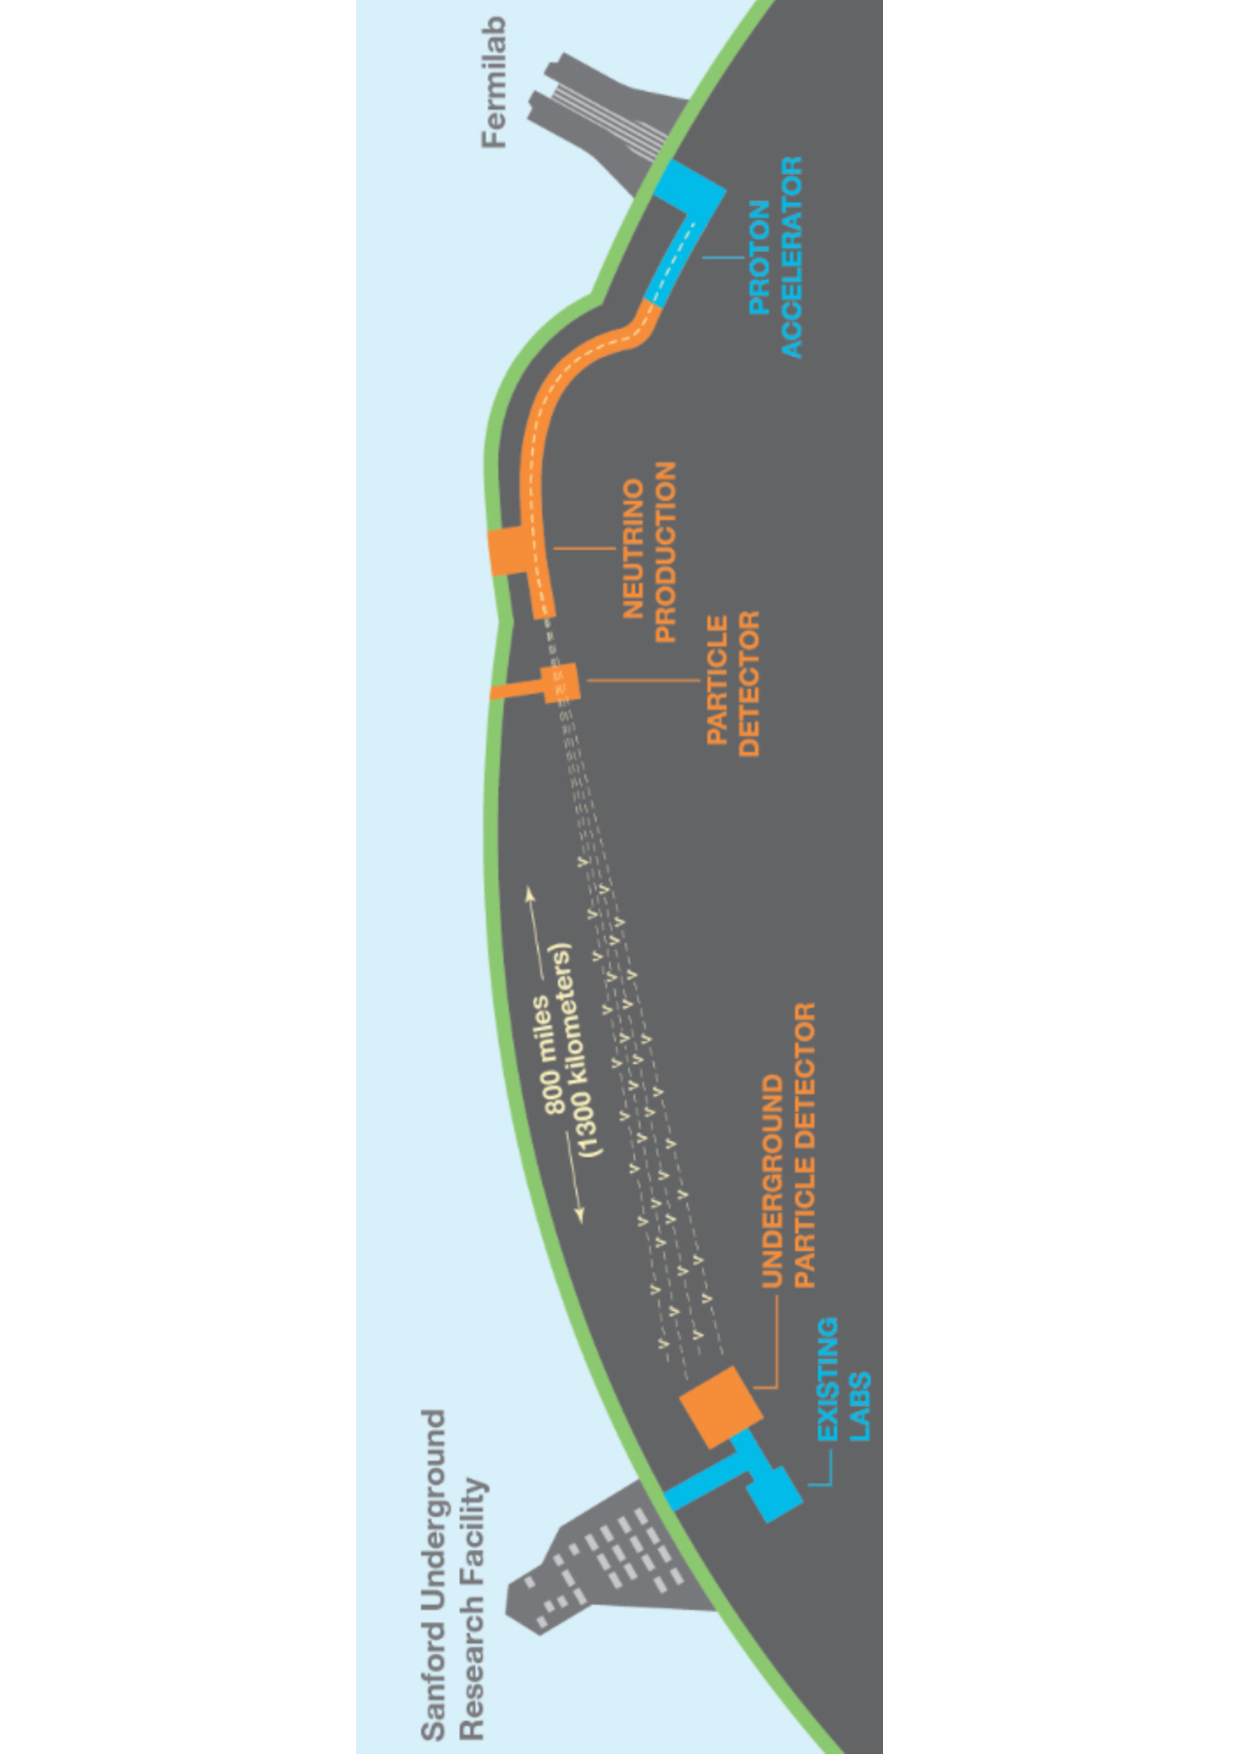
\includegraphics[width=0.9\textwidth]{DUNESchematic}
  \caption[A representation of the DUNE experimental setup]
          {A representation of the DUNE experimental setup. Fermilab, the host lab is shown right. The neutrino beam will be produced at Fermilab, and a high resolution near detector will also be located there. The Stanford Underground Research Facility is shown left, this is 1300 km away from Fermilab, and is where the far detector will be located. Objects in orange need to be built during the lifetime of the experiment, whilst objects in blue already exist. The figure is not to scale. Figure is taken from~\citep{DUNECDR_V1}.}
  \label{fig:DUNESchematic}
\end{figure}

%********************************** %First Section  **************************************
\section{LBNF - the DUNE detector location and neutrino beam} \label{DUNE_LBNF} %Section - X.1 
Formally the far detector site of DUNE, and its associated beam line, do not fall under the remit of the experiment known as DUNE. This is because what may be thought of as the DUNE 'project' is formally split into two separate projects. One of these projects, the experiment called DUNE, is responsible for~\citep{DUNECDR_V1}:
\begin{itemize}
\item The scientific research goals which the experiment aims to accomplish, as well as the program needed to achieve this.
\item The technical requirements needed from the beamline in order to satisfy the physics goals outlined above.
\item The design, building, and maintenance, of the far and near detector systems, in order to achieve the physics program outlined above.  
\end{itemize}
The other project, the Long Baseline Neutrino Facility (LBNF), is responsible for~\citep{DUNECDR_V1}:
\begin{itemize}
\item The design, and construction of a 1.2 MW neutrino beam, utilising the Proton Improvement Plan II (PIP-II) upgrade at Fermilab~\citep{PIP-II}.
\item The civil construction for the near detector site.
\item The excavation of the far detector site, and the preparation of the caverns for the detector modules, including the cryostats and cryogenic systems needed by the DUNE FDs.
\end{itemize}
As such, the design and construction of the neutrino beam, as well as the preparation of both the near and far detector sites, is not within the remit of reponsibility for DUNE, but is instead under the remit of LBNF. This model, whereby there are two separate projects, one repsonsible for the facilities used in the experiment, and another, responsible for the design, construction, and maintainence of the experiments, is the model used at CERN for the LHC, and its experiments. Fermilab as the host lab for LBNF, is thus intimately involved in LBNF, as CERN was in the completion of the LHC. \\

A discussion of the wider DUNE experiment is clearly not possible without first discussing the facilities which LBNF is responsible for building. What follows is thus a brief discussion of the LBNF project. \\

As will be discussed in Section~\ref{sec:DUNEPhys}, DUNE is, first and foremost, a neutrino oscillation experiment, and so it is important to select a far detector location which allows for the largest possible physics opportunities. When a detailed study was performed by the LBNE collaboration to determine the location of the far detector for that experiment, it was determined that the Homestake Mine at SURF was the most optimal site~\citep{LBNEReconfig}. The reason for this was that the steering committee found that with this baseline, it was possible to deliver the full physics potential which LBNE hoped to be able to accomplish, see Section~\ref{sec:DUNEPhys}. The committee further noted that this detector location could be the ``start of a long-term world-leading program...with subsequent phases.'' Following the formation of DUNE, a similar review was performed, and the conclusion reached by this committee was that the FD site chosen by LBNE was also the location at which DUNE could best achieve its physics goals. This determination was made under the remit that the subsequent phases outlined by the LBNE reconfiguration report were performed. These were that a highly capable near detector is built, that the FD consists of at least 35 kton at the 4850 ft level, and that a multi-MW beamline is used. \\

SURF is located in Lead, South Dakota, and is the refurbished Homestake gold mine. Upon mining operations finishing, the mine became briefly disused before being reopened as the Deep Underground Science and Engineering Laboratory (DUSEL). When funding for DUSEL ceased, the US Department of Energy (DOE), through Lawrence Berkley National Lab agreed to support ongoing research efforts~\citep{SURFWebsite}. DUNE will be located near the Ross shaft, one of two shafts which go to the 4850 level. Near the other shaft, the Yates Shaft, is what is now called the Davis Campus, named after Ray Davis who performed the experiment bearing his name at the Homestake mine in the late 1960's~\citep{RayDavis1968, RayDavis1988}. \\

In order to prepare SURF for an experiment of the size of DUNE, a major renovation effort is required. This is because both shafts down to the 4850 need to be reinforced to be able to cope with the amount of rock which has to be excavated, and the amount of building materials which need to brought down to the 4850 level to build the DUNE detectors, and cryogenic equipment~\citep{DUNECDR_V3}. Before excavation could occur extensives studies were required, this was to ensure that rock around the proposed cavern system is of high enough quality to accomadate the cavern system required for DUNE. These studies confirmed that the chosen site was suitable~\citep{DUNECDR_V3}. \\

The dimsensions of the cavern system which need to be excavated in order to accomodate the DUNE detectors is shown in Figure~\ref{fig:DUNECavernSystem}. From Figure~\ref{fig:DUNECavernSystem} it can be seen that the DUNE FDs will be located in two large caverns, either side of a central reservation, with each cavern housing two detector pits. Each detector will be contained within a self-standing, steel framed structure, within this structure will be a membrane cryostat which will house a total of 17.1 kt of LAr~\citep{DUNECDR_V1}. Further information regarding the DUNE FDs can be found in Section~\ref{sec:DUNEDetector}. \\

\begin{figure}[h!]
  \centering
  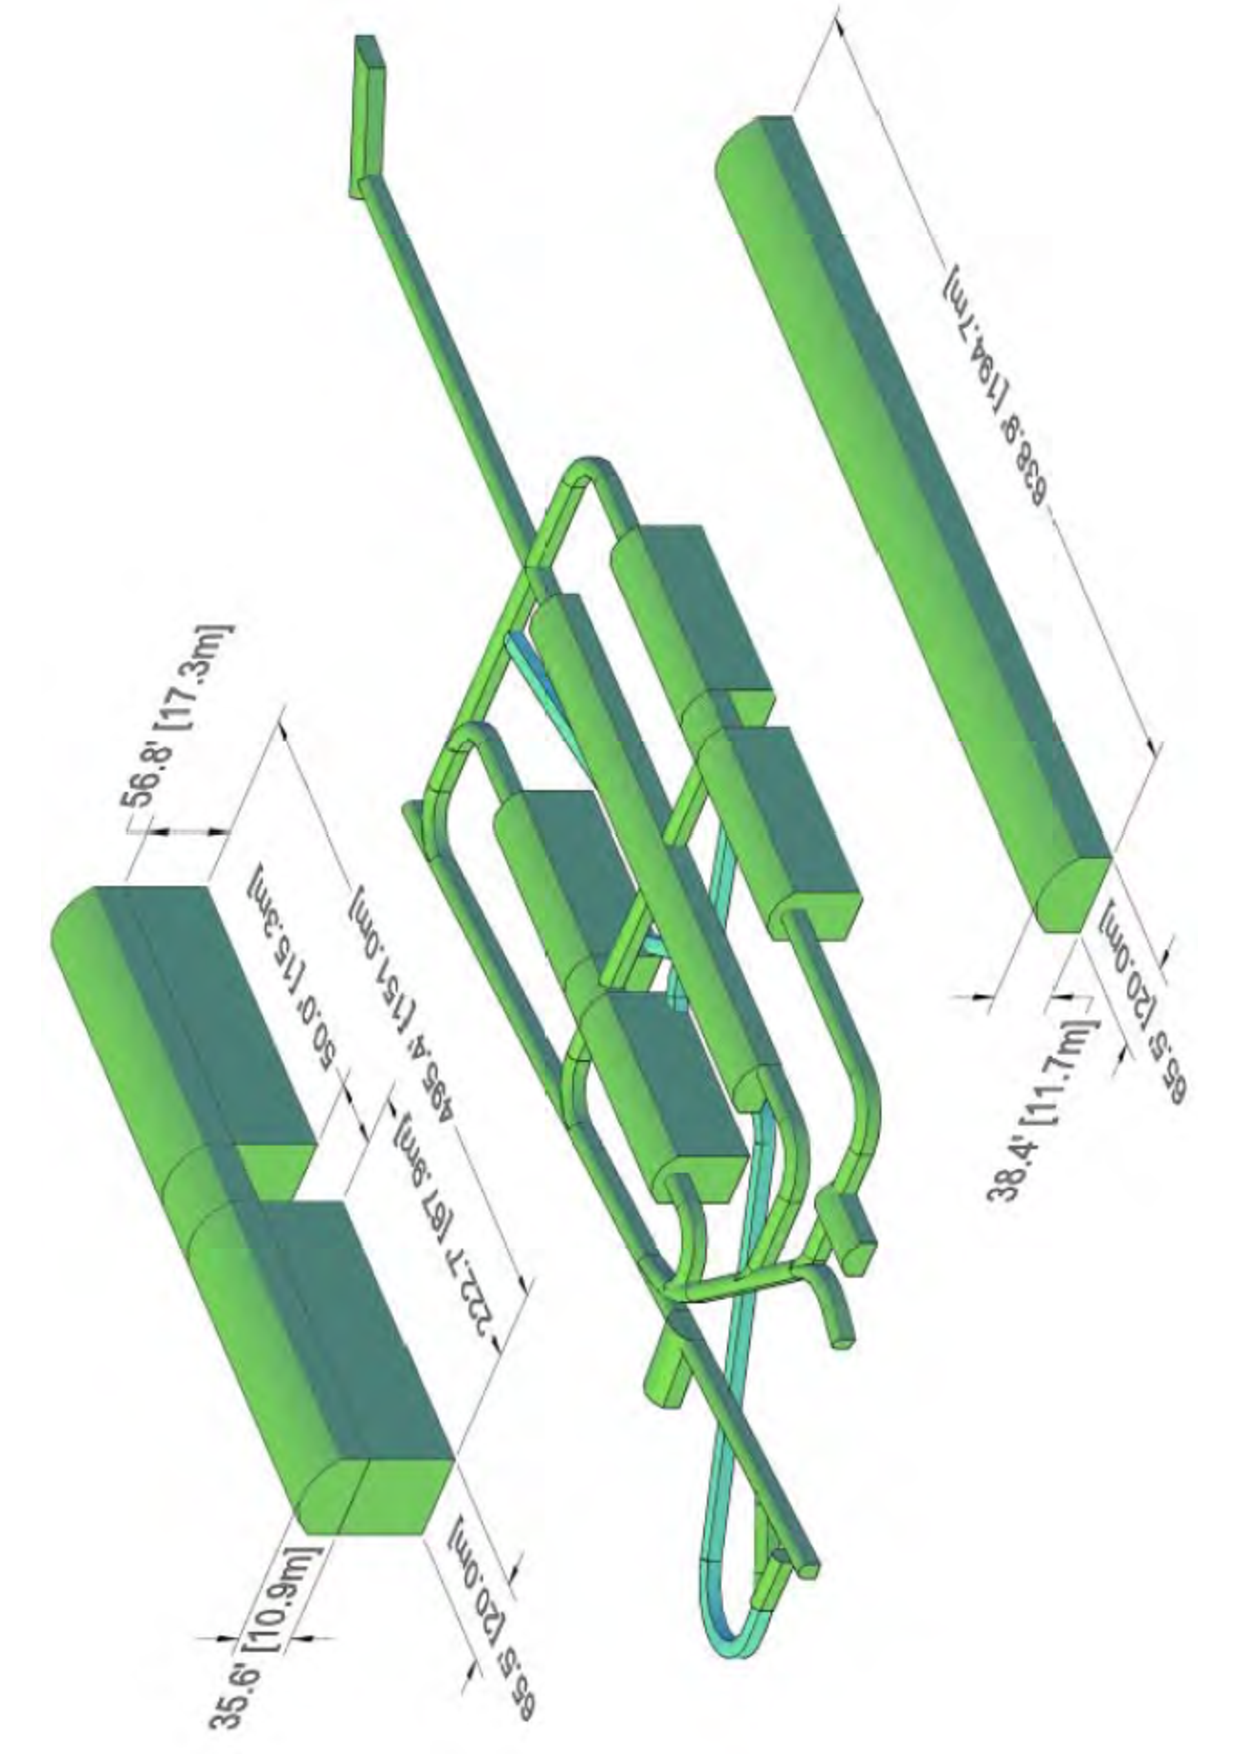
\includegraphics[width=0.7\textwidth]{DUNECavernSystem}
  \caption[A representation of the future LBNF cavern system at SURF, which DUNE will use]
          {A representation of the future LBNF cavern system at SURF, which DUNE will use. The top of the figure shows one of the main caverns, composed of two detector pits. The centre of the figure shows the entire cavern system, whilst the bottom of the figure shows area which will house the cryogenic equipment. All caverns shown need to be excavated. The Ross Shaft is located a small distance from the bottom left corner of the figure. The Yates Shaft is located roughly 1 km from the cavern system, in the direction of the top left hand corner of the figure. The dimensions shown are estimations, and the final dimensions may be slightly smaller. The figure is taken from~\citep{DUNECDR_V3}.}
  \label{fig:DUNECavernSystem}
\end{figure}

The other remit of LBNF, is the design and construction of the beam line, as well as the providing the facilities to house the DUNE ND. A schematic showing the near site facilities which will be built by LBNF, is shown in Figure~\ref{fig:DUNENearDetectorComplex}. From Figure~\ref{fig:DUNENearDetectorComplex}, it can be seen that upon extraction from the Main Injector, the proton beam will be sent through a man-made embankment, the height of which will be approximately 18 m. This proton beam will then be bent 7.2$^{\circ}$ westward, and 5.8$^{\circ}$ downwards, so as to point at a target, which will allow for the neutrino beam to be pointed towards the FD location at SURF. Upon the protons hitting the target, mesons will be produced which will be focused by a set of magentic horns. As these mesons decay in the 'decay pipe' they will produce neutrinos, it is these neutrinos which will be measured at the FD site. The energies of the neutrinos produced are between 0.5 and 5 GeV, this allows for a wide band neutrino beam to be used. The advantage of using a wide band neutrino beam is that the DUNE FD can then observe the maxima from the both the first and second oscillation maxima, at approximately 2.4 and 0.8 GeV. The reference design for the 'decay pipe' is 194 m long and filled with Helium. Studies are on-going to determine the most optimal separation of the beam-horns, and the most optimal length of the decay pipe~\citep{DUNECDR_V2, DUNECDR_V3}. At the end of the 'decay pipe' is an 'absorber' which will absorb any hadrons which have not decayed. \\

\begin{figure}[h!]
  \centering
  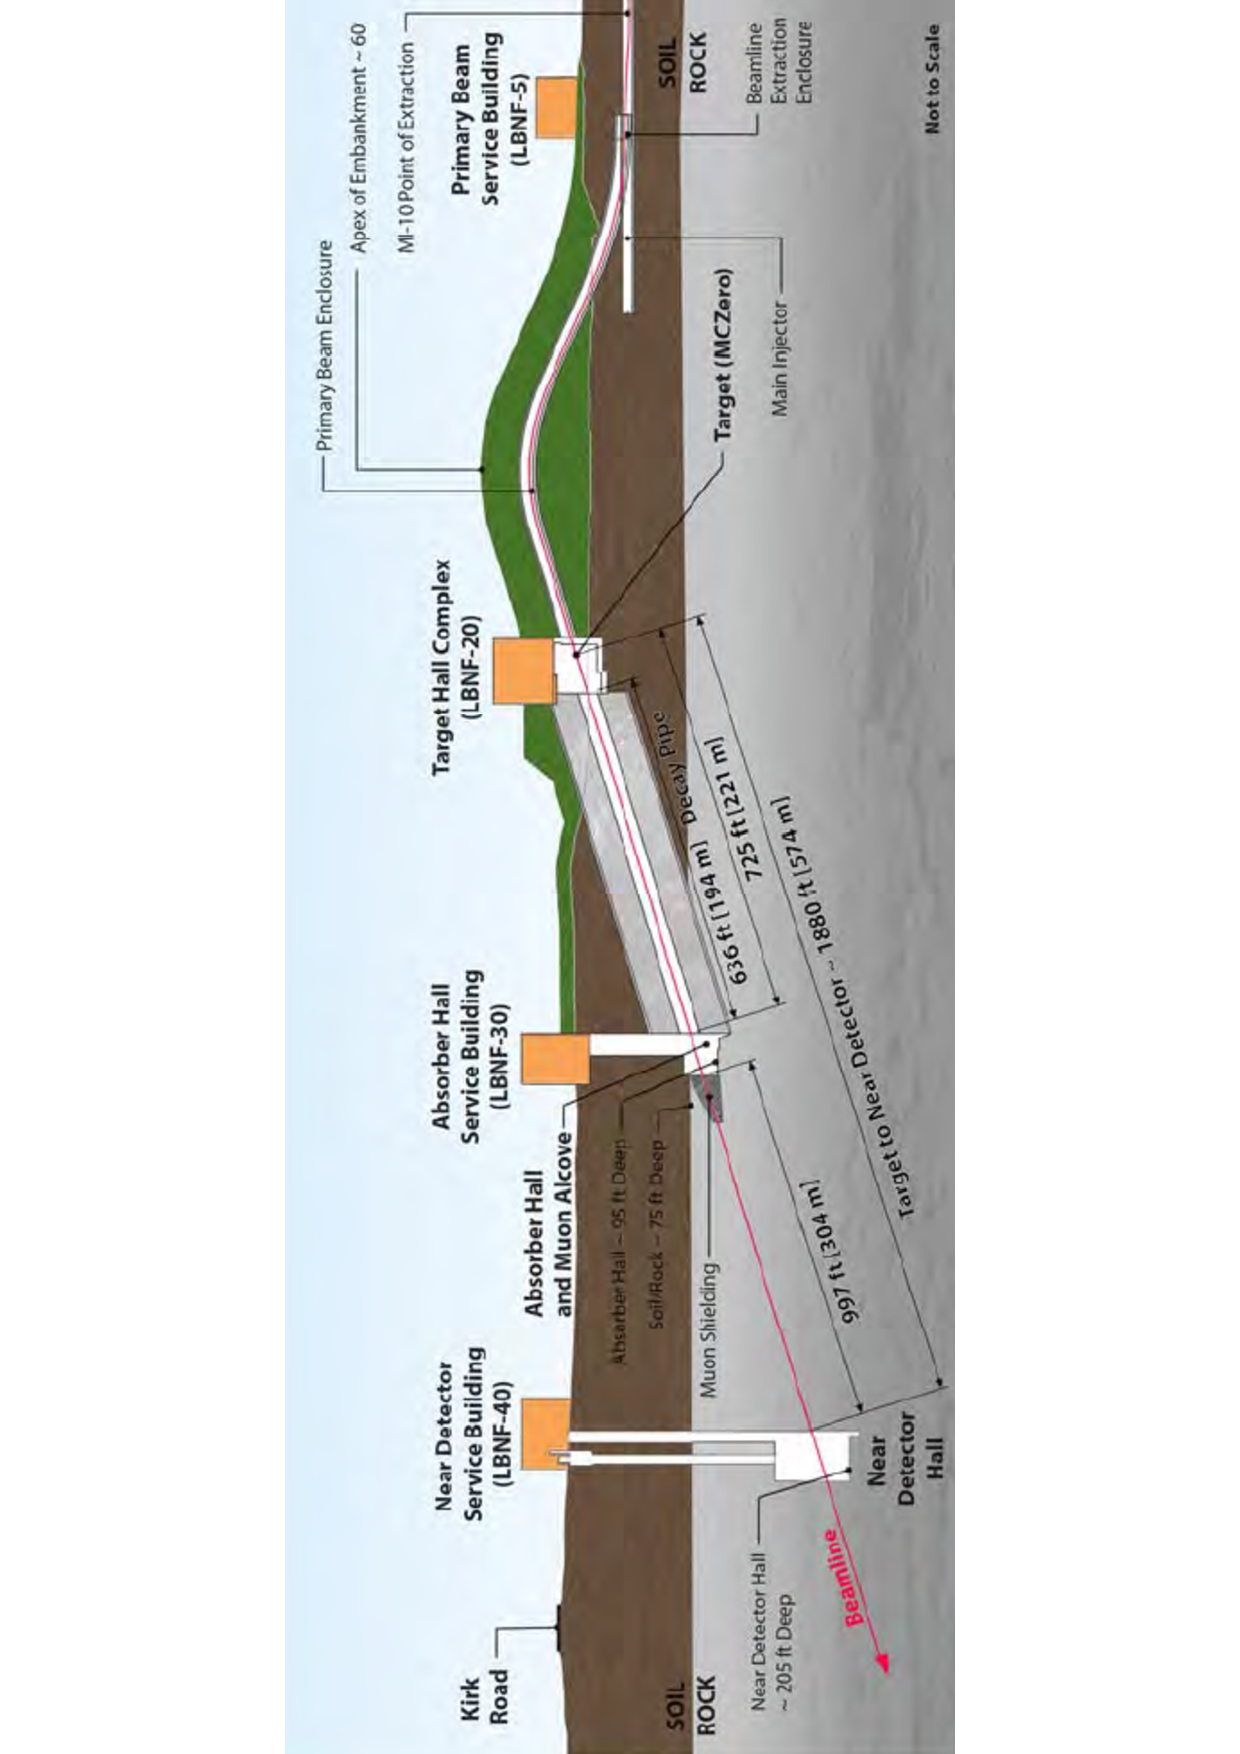
\includegraphics[width=0.9\textwidth]{NearDetectorComplex}
  \caption[A representation of the future LBNF near site at Fermilab, which DUNE will use]
          {A representation of the future LBNF near site at Fermilab, which DUNE will use. From right to left, the beam extraction point, man-made hill, target hall complex, meson decay pipe, absorber hall, and the near detector hall can be seen. Measurements are shown for the decay pipe (a reference design, top, and an alternative design, bottom), and the distance between the absorber and near detector are shown, though the figure is not to scale. All facilities need to built, including the extraction point from the Main Injector, and the man-made hill. The figure is taken from~\citep{DUNECDR_V3}.}
  \label{fig:DUNENearDetectorComplex}
\end{figure}

The beamline illustrated above will utilise the Main Injector beamline after the PIP-II upgrade~\citep{PIP-II}, whereby protons will be delivered with energies between 60 and 120 GeV, corresponding to a beam power of 1.0 to 1.2 MW. The ability to vary the beam power will give DUNE the ability to optimise the flux spectrum, and to better understand the systematic effects of the beam~\citep{DUNECDR_V1}. \\

Also associated with the near site, is the construction of the DUNE ND. The distance between the ND and the abosrber hall will be a minimum of 210 m, due to the muon-range-out distance, and is 304 m in the reference design~\citep{DUNECDR_V3}. The DUNE ND will be comprised of at least one detector, the exact details of the ND are covered in Section~\ref{sec:DUNEDetector_Near}, where the various detector technologies currently being considered are discussed. \\

%********************************** %Third Section  *************************************
\section{The physics capabilities of DUNE} \label{sec:DUNEPhys}%Section - X.2
As mentioned above, DUNE hopes to be able to have a wide ranging physics program. These topics include, but are not limited to, precision measurements of neutrino oscillation physics, discussed in Section~\ref{sec:DUNEPhys_Neut}, searching for nucelon decay in several important decay modes, discussed in Section~\ref{sec:DUNE_NDK}, and the detection and measurement of the $\nu_e$ flux from a core-collapse supernovae in our galaxy, should one occur, this is discussed in Section~\ref{sec:DUNE_Other}. \\

%********************************** % 3.1 Section  *************************************
\subsection{Neutrino physics} \label{sec:DUNEPhys_Neut} %Section - X.2.1
The primary goals of DUNE concern neutrino physics, many of these ideas were introduced in Section~\ref{sec:NeutPhys}. The primary goals of DUNE are outlined now, and illustrated more fully below~\citep{DUNECDR_V2}:
\begin{itemize}
\item Determine the neutrino mass hierachy.
\item Measure the charge-parity (CP) violating phase - $\delta_{CP}$.
\item Make precision measurements of the neutrino mixing parameters, such as $\theta_{13}$, $\theta_{23}$, and $\Delta m^{2}_{31}$.
\end{itemize}
There are also secondary physics goals concerning neutrino physics, these include:
\begin{itemize}
\item Measuring the rate of $\nu_{\tau}$ appearance.
\item Measuring neutrino oscillations using atmospheric neutrinos.
\item Measuring a wide range of neutrino cross-sections, using the ND.
\item Measuring nuclear effects, particularly neutrino final-state interaction, using the ND.
\end{itemize}

As presented in Section~\ref{sec:NeutPhys}, both the matter effect, and $\delta_{CP}$ introduce an asymettry between neutrino and anti-neutrino oscillations. As the matter effect is caused by the difference in the presence/absence of electrons/positrons in the Earth, it increases with distance. The result of this is that for baselines longer than approximately 1000 km the two effects can be resolved~\citep{Bass:2013vcg}. It is for this reason that with a baseline of 1300 km, DUNE will be able to unambiguously determine the neutrino mass hierarchy and determine $\delta_{CP}$~\citep{Diwan:2004bt}. \\

The reason for requiring a broadband neutrino beam can be seen in Figure~\ref{fig:DUNEOscillProb}, where it can be seen that whilst the energy of the first neutrino oscillation maxima is relatively unaffected by the value of $\delta_{CP}$, the energies of the higher oscillation maxima are strongly affected by the value of $\delta_{CP}$. The result of this, is that it is vital that DUNE is able to accurately the measure the rate of $\nu_e$ appearence to the lowest energies of the neutrino beam it recieves from LBNF. It can also be seen taht there are larrge differences in the expected oscillation probabilities for neutrinos and anti-neutrinos, therefore in order to measure the effect of $\delta_{CP}$, the beam from LBNF will also have to be able to operate in both neutrino and anti-neutrino mode. \\

\begin{figure}[h!]
  \centering
  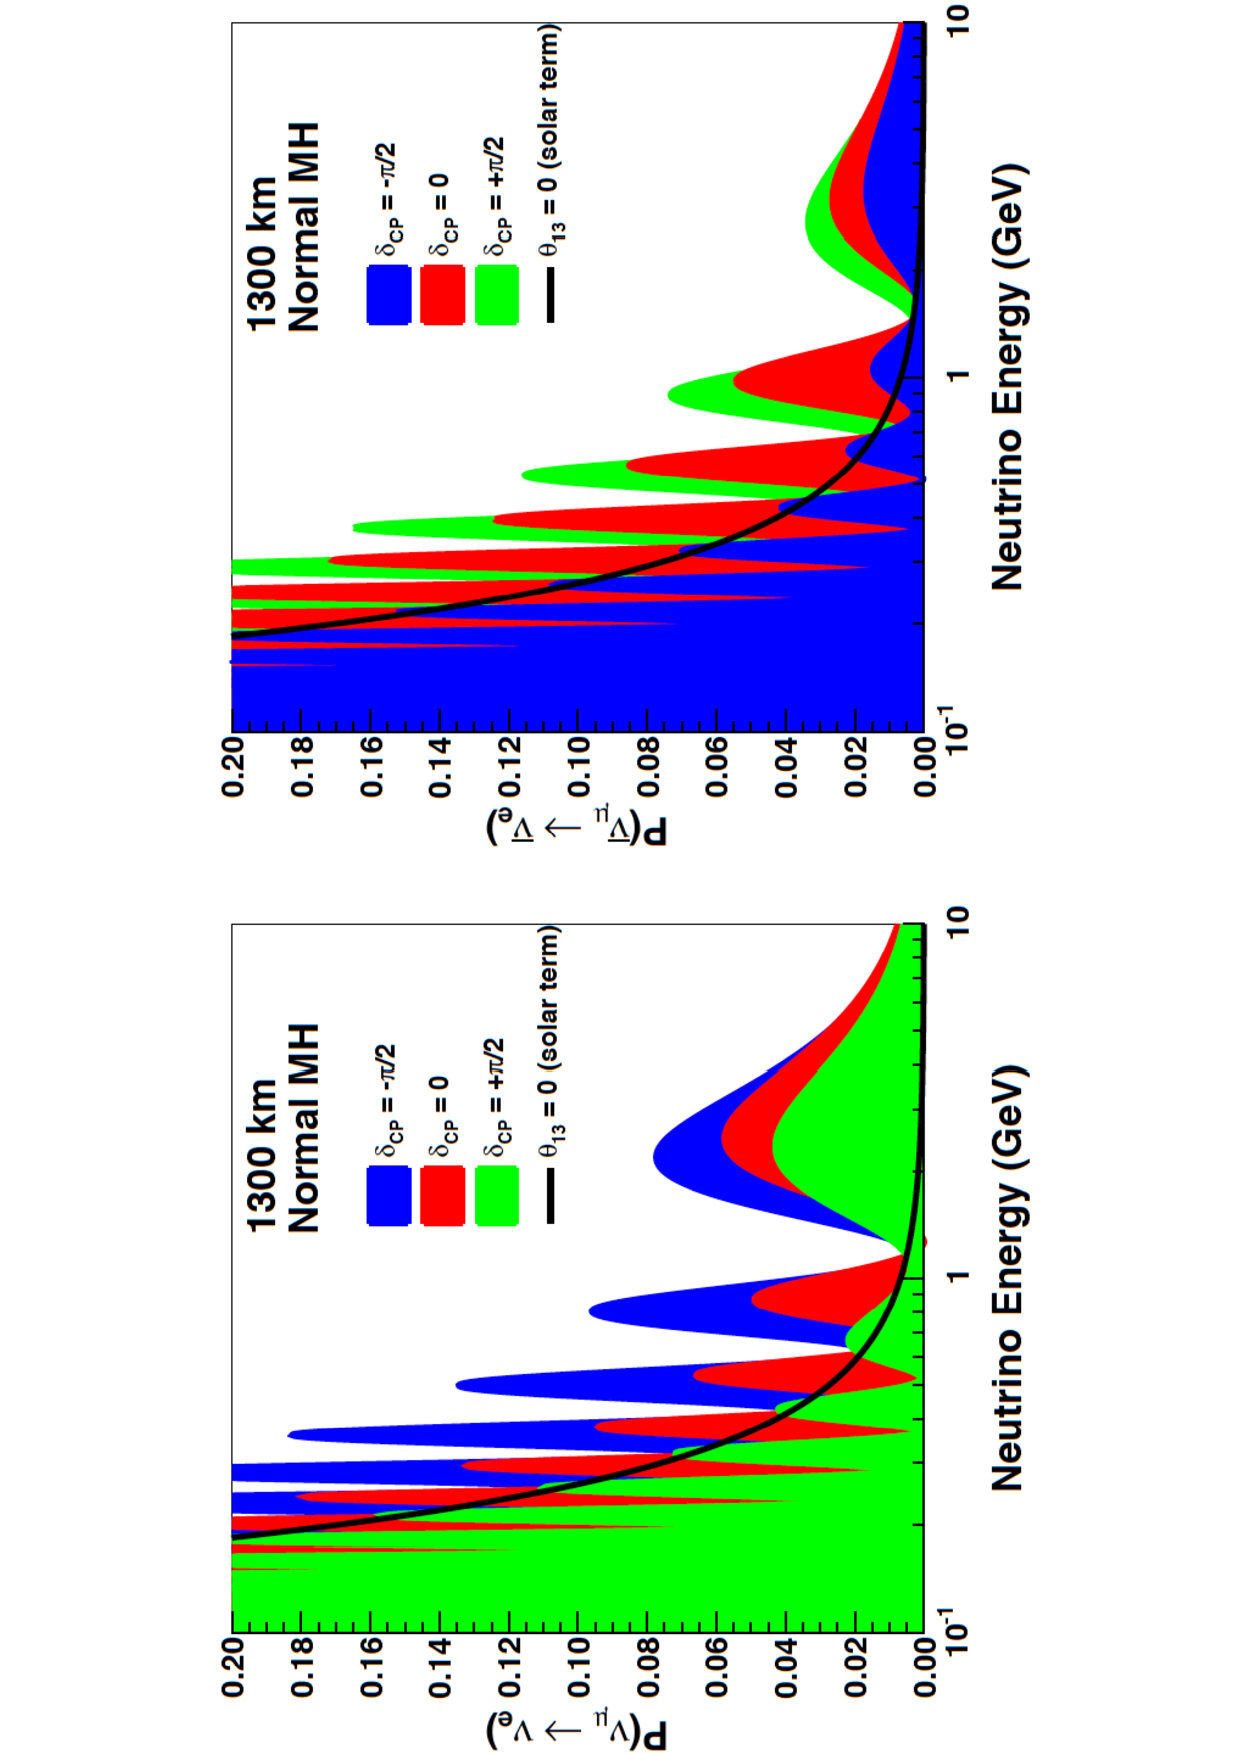
\includegraphics[width=0.9\textwidth]{DUNEOscillProb}
  \caption[The $\nu_e$ appearence probability at 1300 km, as a function of neutrino energy, for a range of values of $\delta_{CP}$]
          {The $\nu_e$ appearence probability at 1300 km, as a function of neutrino energy, for a range of values of $\delta_{CP}$. Left shows the probabilities for neutrinos, whilst right shows the probabilities for anti-neutrinos. Both figures assume normal mass hierarchy ($\nu_e$ is the lightest state). The probabilites for different values of $\delta_{CP}$ are shown, $\delta_{CP} = -\pi/2$ (blue), $\delta_{CP} = 0$ (red), $\delta_{CP} = \pi/2$ (green). The figure is taken from~\citep{DUNECDR_V2}.}
  \label{fig:DUNEOscillProb}
\end{figure}

When presenting the DUNE sensitivities to the determinations of the mass hierarchy, and the value of $\delta_{CP}$, the figures are shown with exposures of 300 kt MW yrs. This exposure represents seven years of data taking with a 40 kt detector, and a 1.07 MW beam, where the seven years of data is equally split between the neutrino and anti-neutrino modes. In all plots, two possible beam configurations are shown, the reference design which was outlined in Section~\ref{DUNE_LBNF}, and an optimized design~\citep{DUNECDR_V3}. The measurements of both the mass hierarchy and the value of $\delta_{CP}$ are sensitive to the true values of $\sin^2\theta_{13}$, $\sin^2\theta_{23}$, and $\Delta m^{2}_{31}$, and so have been fixed to be 0.085, 0.45, and 2.46 $\times$ 10$^{-3}$ eV$^{2}$, respectively. \\

Figure~\ref{fig:DUNEMassHierarchy} shows the significance with which DUNE will be able to determine the neutrino mass hierarchy for all values of $\delta_{CP}$. It can be seen that the mass hierarchy can be determined with a significance of $\sqrt{\bar{\Delta{\chi^2}}}$ = 5 for almost all values of $\delta_{CP}$ with the reference beam design. It can also be seen that the mass hierarchy can be more conclusively determined if the hierarchy is inverted. \\

\begin{figure}[h!]
  \centering
  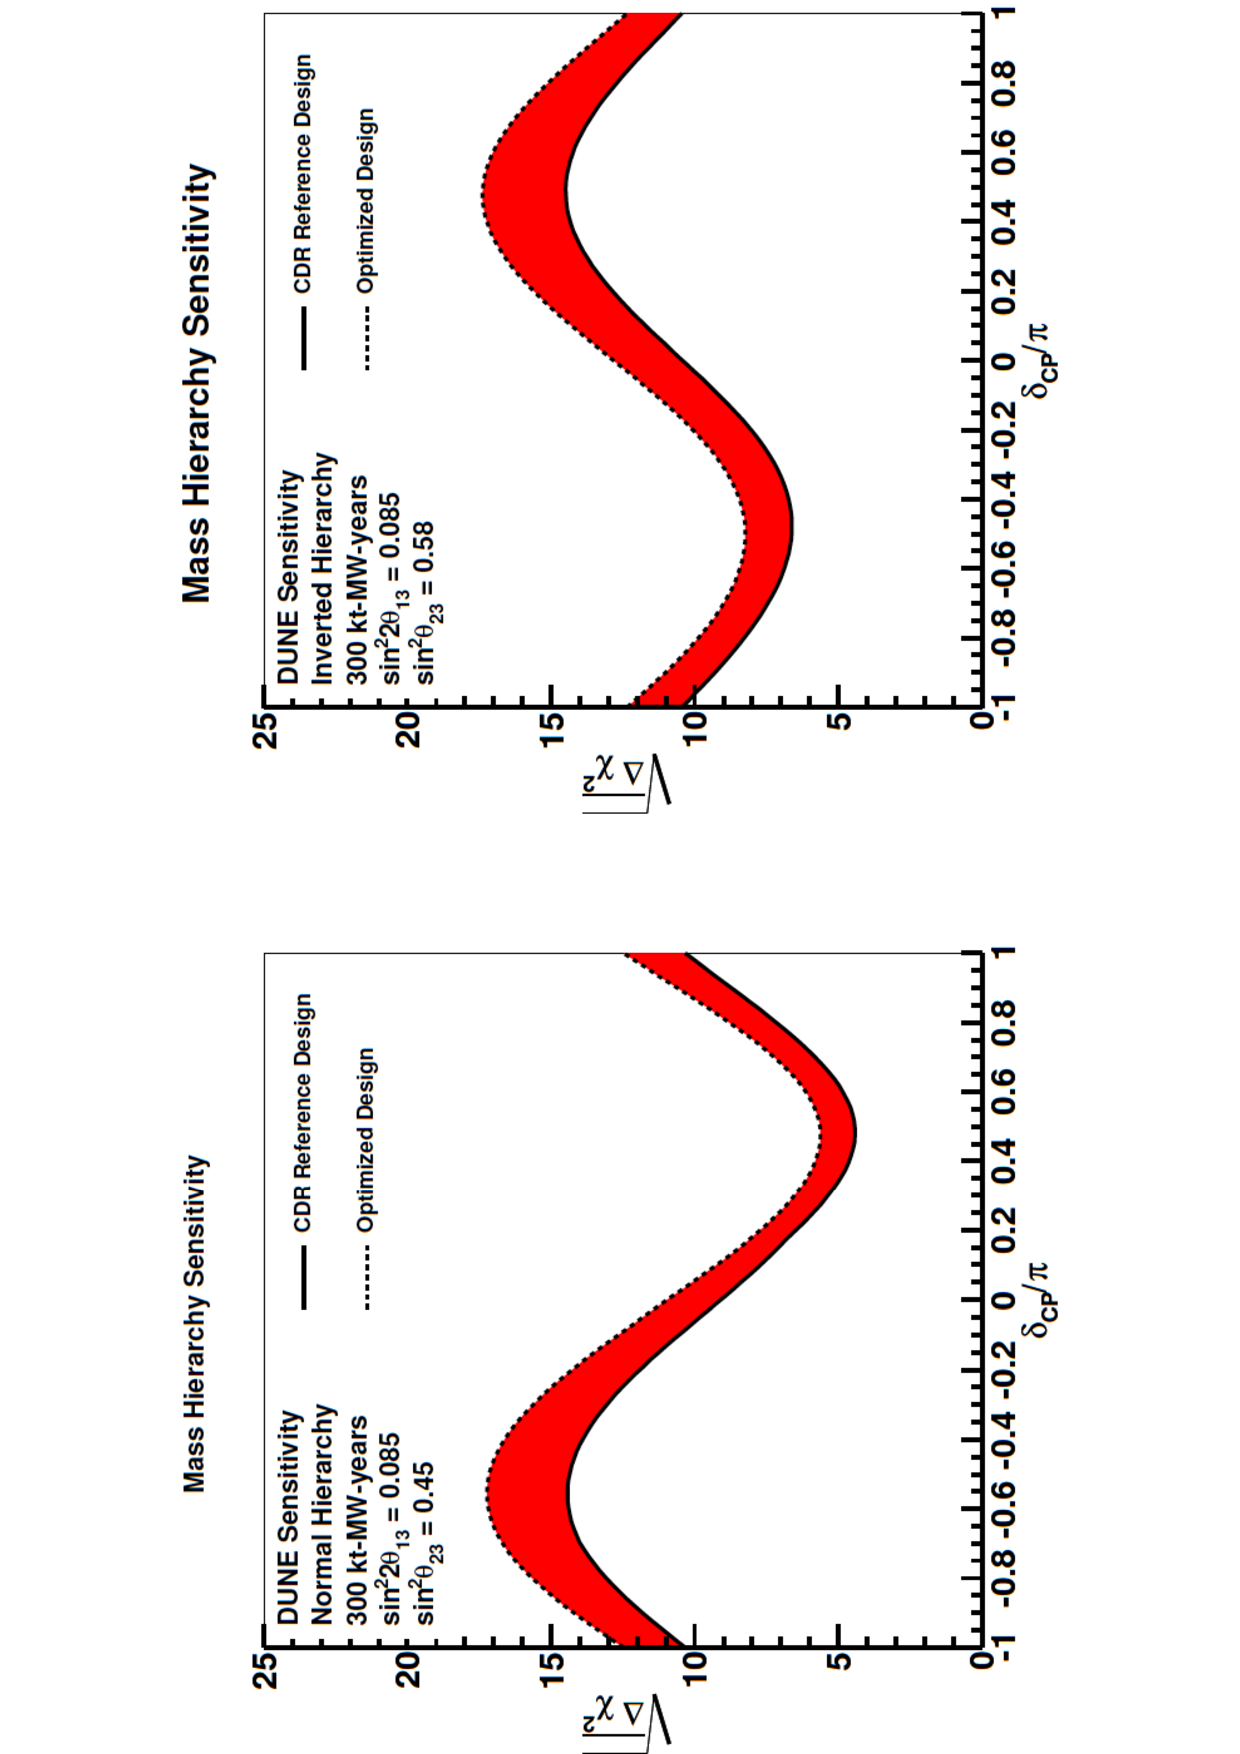
\includegraphics[width=0.9\textwidth]{DUNEMassHierarchy}
  \caption[The significance with which DUNE will be able to determine the neutrino mass hierarchy for all values of $\delta_{CP}$]
          {The significance with which DUNE will be able to determine the neutrino mass hierarchy for all values of $\delta_{CP}$. Left shows the senstivity assuming the normal hierarchy, whilst right shows the sensitivities assuming the inverted hierarchy. The variation in the proposed beam design is shown by the shaded region. The figure is taken from~\citep{DUNECDR_V2}.}
  \label{fig:DUNEMassHierarchy}
\end{figure}

Figure~\ref{fig:DUNECPViolation} shows the significance with which DUNE will be able to determine the value of $\delta_{CP}$ for all values of $\delta_{CP}$. It can be seen that even with 7 years worth of data there are regions where the value of $\delta_{CP}$ cannot be determined accurately, this is because if $\delta_{CP}$ equals $-\pi$, 0, or $\pi$ there would be no CP-violation. Therefore, for values of $\delta_{CP}$ around these values, the significance to which $\delta_{CP}$ can be determined must approach 0. As such, even at very large exposures of 1320 kt MW yr, only 75\% of the $\delta_{CP}$ values can be determined to a significance of 3$\sigma$~\citep{DUNECDR_V2} using the reference beam design. However, even with the modest exposure of 300 kt MW yr, DUNE can determine the value of $\delta_{CP}$ for over 50\% of the values for $\delta_{CP}$ to a significance of 3$\sigma$ using the reference beam design. This shows the difficulty associated with determining the value of $\delta_{CP}$ should it be close to any the CP-conserving values of $\delta_{CP}$. \\

\begin{figure}[h!]
  \centering
  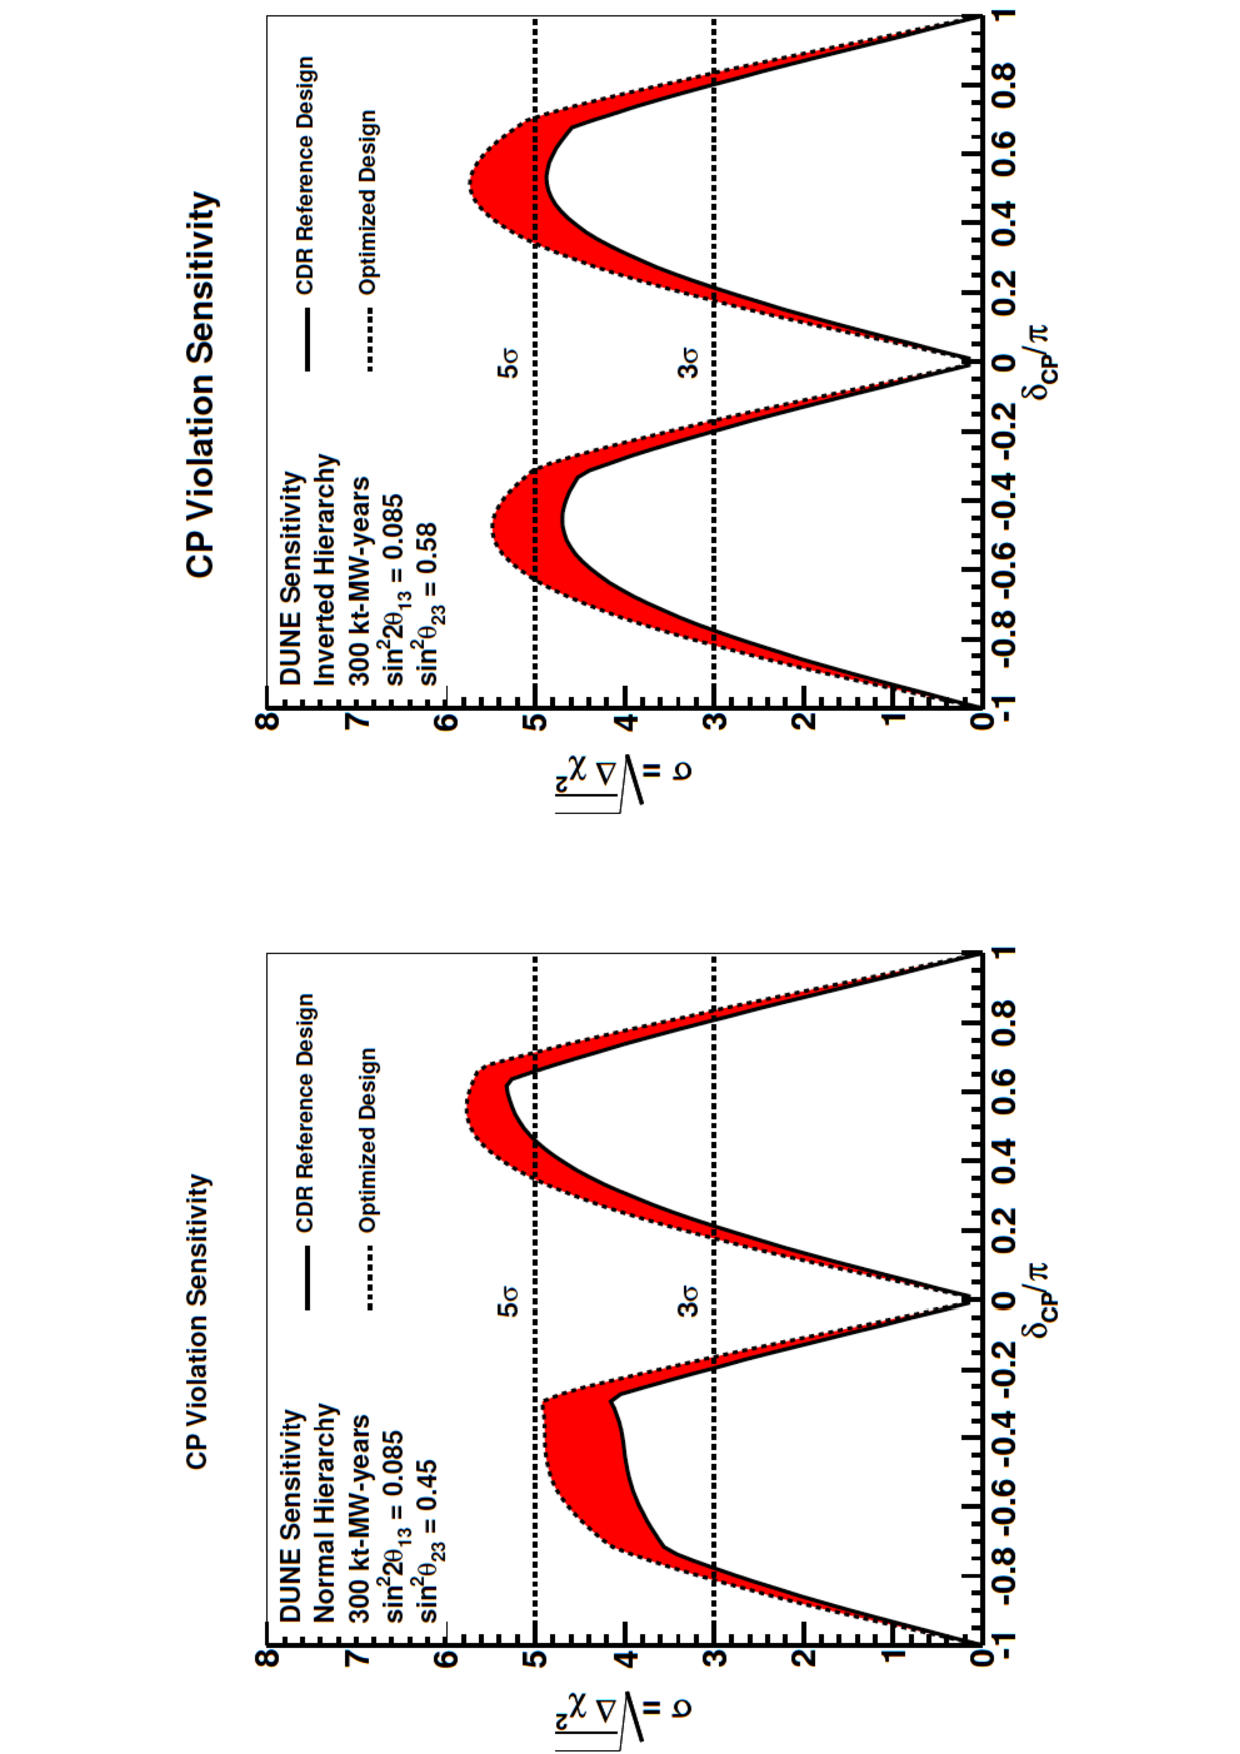
\includegraphics[width=0.9\textwidth]{DUNECPViolation}
  \caption[The significance with which DUNE will be able to determine the value of $\delta_{CP}$ for all values of $\delta_{CP}$]
          {The significance with which DUNE will be able to determine the value of $\delta_{CP}$ for all values of $\delta_{CP}$. Left shows the senstivity assuming the normal hierarchy, whilst right shows the sensitivities assuming the inverted hierarchy. The variation in the proposed beam design is shown by the shaded region. The figure is taken from~\citep{DUNECDR_V2}.}
  \label{fig:DUNECPViolation}
\end{figure}

Given the structure of Figure~\ref{fig:DUNECPViolation}, it can be instructive to instead observe the resolution to which the value of $\delta_{CP}$ can be determined with increasing exposures, this is shown in Figure~\ref{fig:DUNECPViolationRes}. Figure~\ref{fig:DUNECPViolationRes} shows curves for the cases when the value of $\delta_{CP}$ is both maximally CP-violating ($\delta_{CP}$ = 90$^{\circ}$), and CP-conserving ($\delta_{CP}$ = 0$^{\circ}$). Somewhat paradoxically, the resolution is better when $\delta_{CP}$ = 0$^{\circ}$, the reason for this is that the region of values of $\delta_{CP}$ for which CP-violation would not be observed, becomes increasingly small as exposure increases. This means that the resolution to which $\delta_{CP}$ can be determines becomes more accurate. However, the more interesting result would be the one which supported $\delta_{CP}$ having a value which causes maximal CP-violation. \\

\begin{figure}[h!]
  \centering
  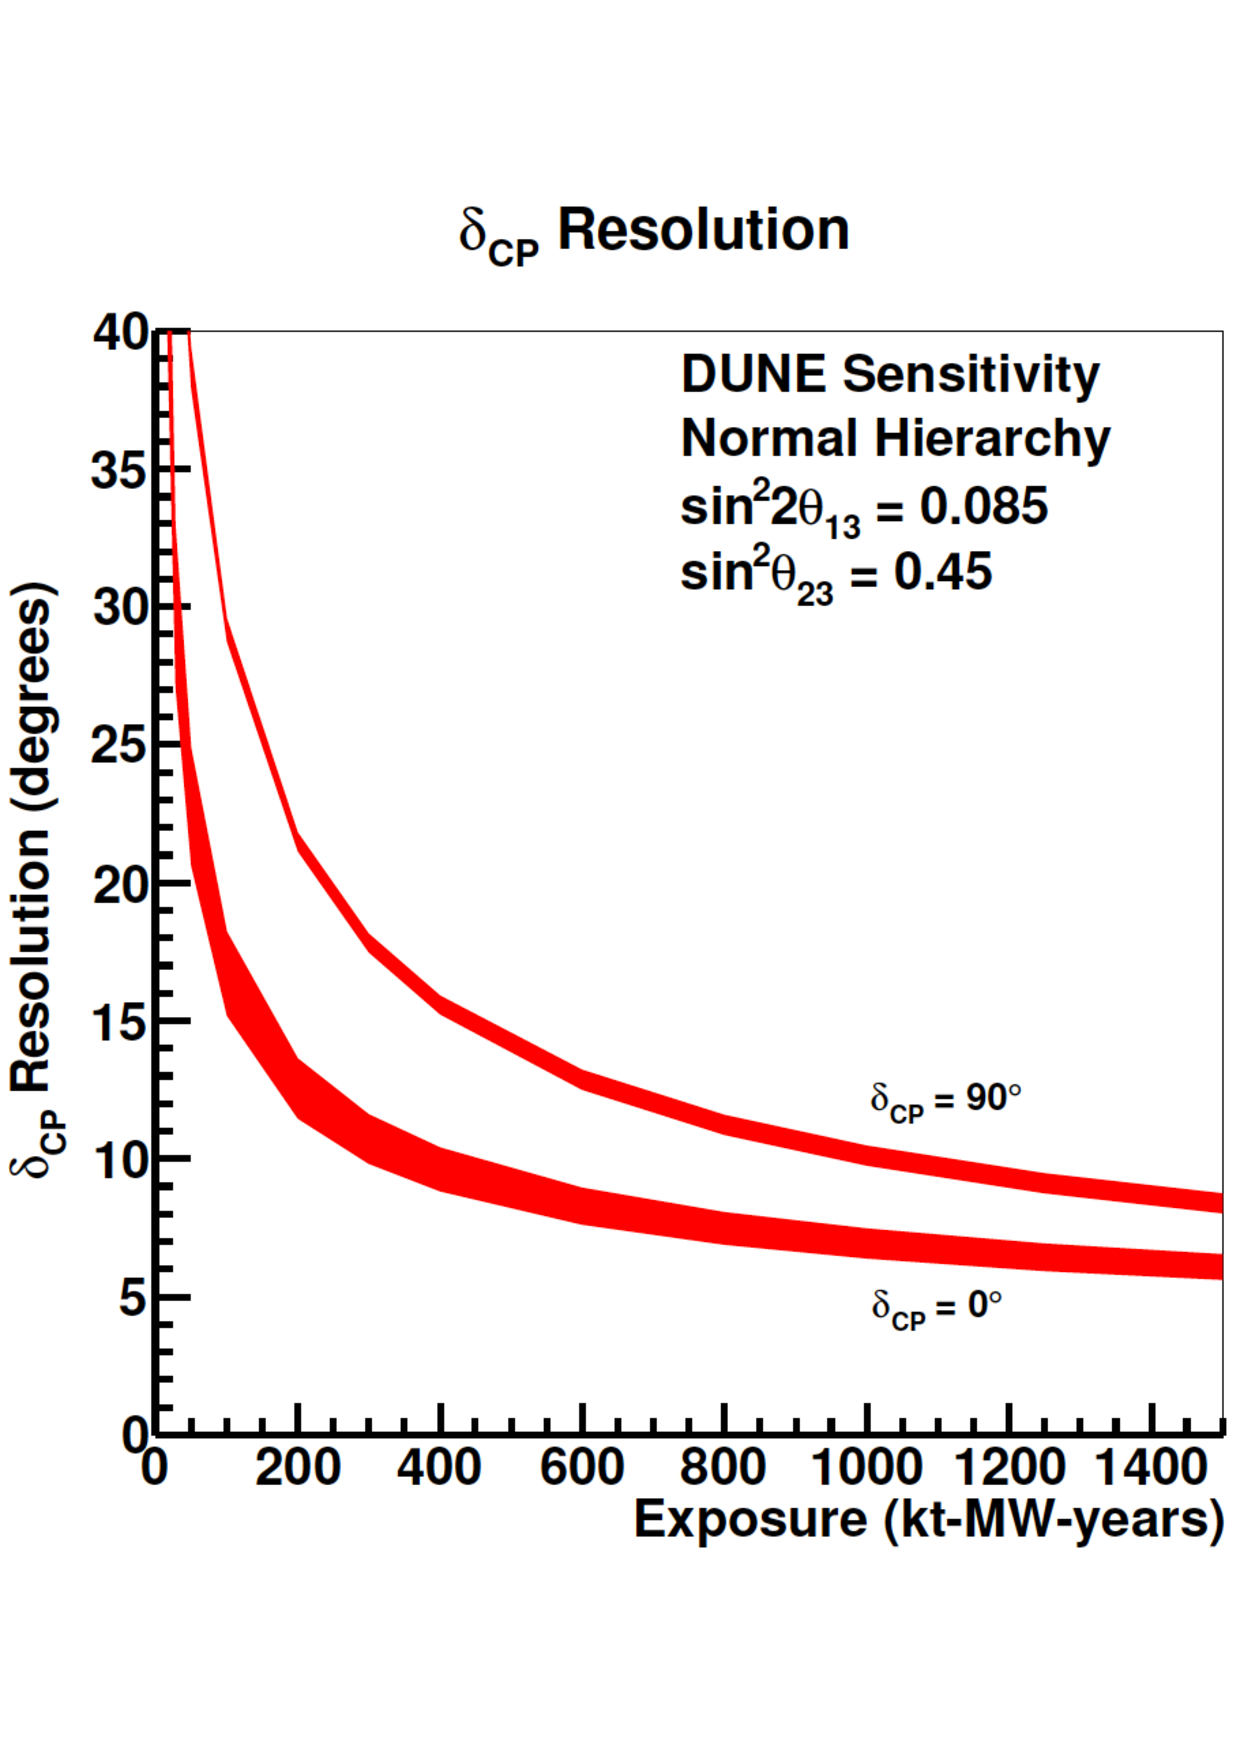
\includegraphics[width=0.5\textwidth]{DUNECPViolationRes}
  \caption[The resolution with which DUNE will be able to determine the value of $\delta_{CP}$ for increasing exposures]
          {The resolution with which DUNE will be able to determine the value of $\delta_{CP}$ for increasing exposures. Two bands are shown, one for a value of $\delta_{CP}$ which could cause maximal CP-violation ($\delta_{CP}$ = 90$^{\circ}$), and another where there would be no CP-violation ($\delta_{CP}$ = 0$^{\circ}$). A normal hierarchy is assumed, and the bands show the sensitivities to the potential beam designs. The figure is taken from~\citep{DUNECDR_V2}.}
  \label{fig:DUNECPViolationRes}
\end{figure}

DUNE also aims to perform precision measurements of the neutrino mixing parameters in order to improve sensitivity to any physics beyong the standard thee-flavour oscillation model. As discussed in Section~\ref{sec:NeutPhys}, the current best limit for the value of $\theta_{23}$ does not determine which octant it is in, specifically whether it is more, or less than 45$^{\circ}$. Determining the octant of $\theta_{23}$ is important, as should it be found that $\theta_{23}$ is equal to 45$^{\circ}$ it would hint an unkown symmetry. DUNE will determine the value of $\theta_{23}$ by combining measurements of $\nu_{\mu} \rightarrow \nu_{\mu}$ and $\nu_{\mu} \rightarrow \nu_{e}$, which are sensitive to $\sin^{2}2\theta_{23}$ and $\sin^2\theta_{23}$ respectively. Figure~\ref{fig:DUNEOctantDetermination} shows the significance to which the octant of $\theta_{23}$ can be determined for different values of $\theta_{23}$. \\

\begin{figure}[h!]
  \centering
  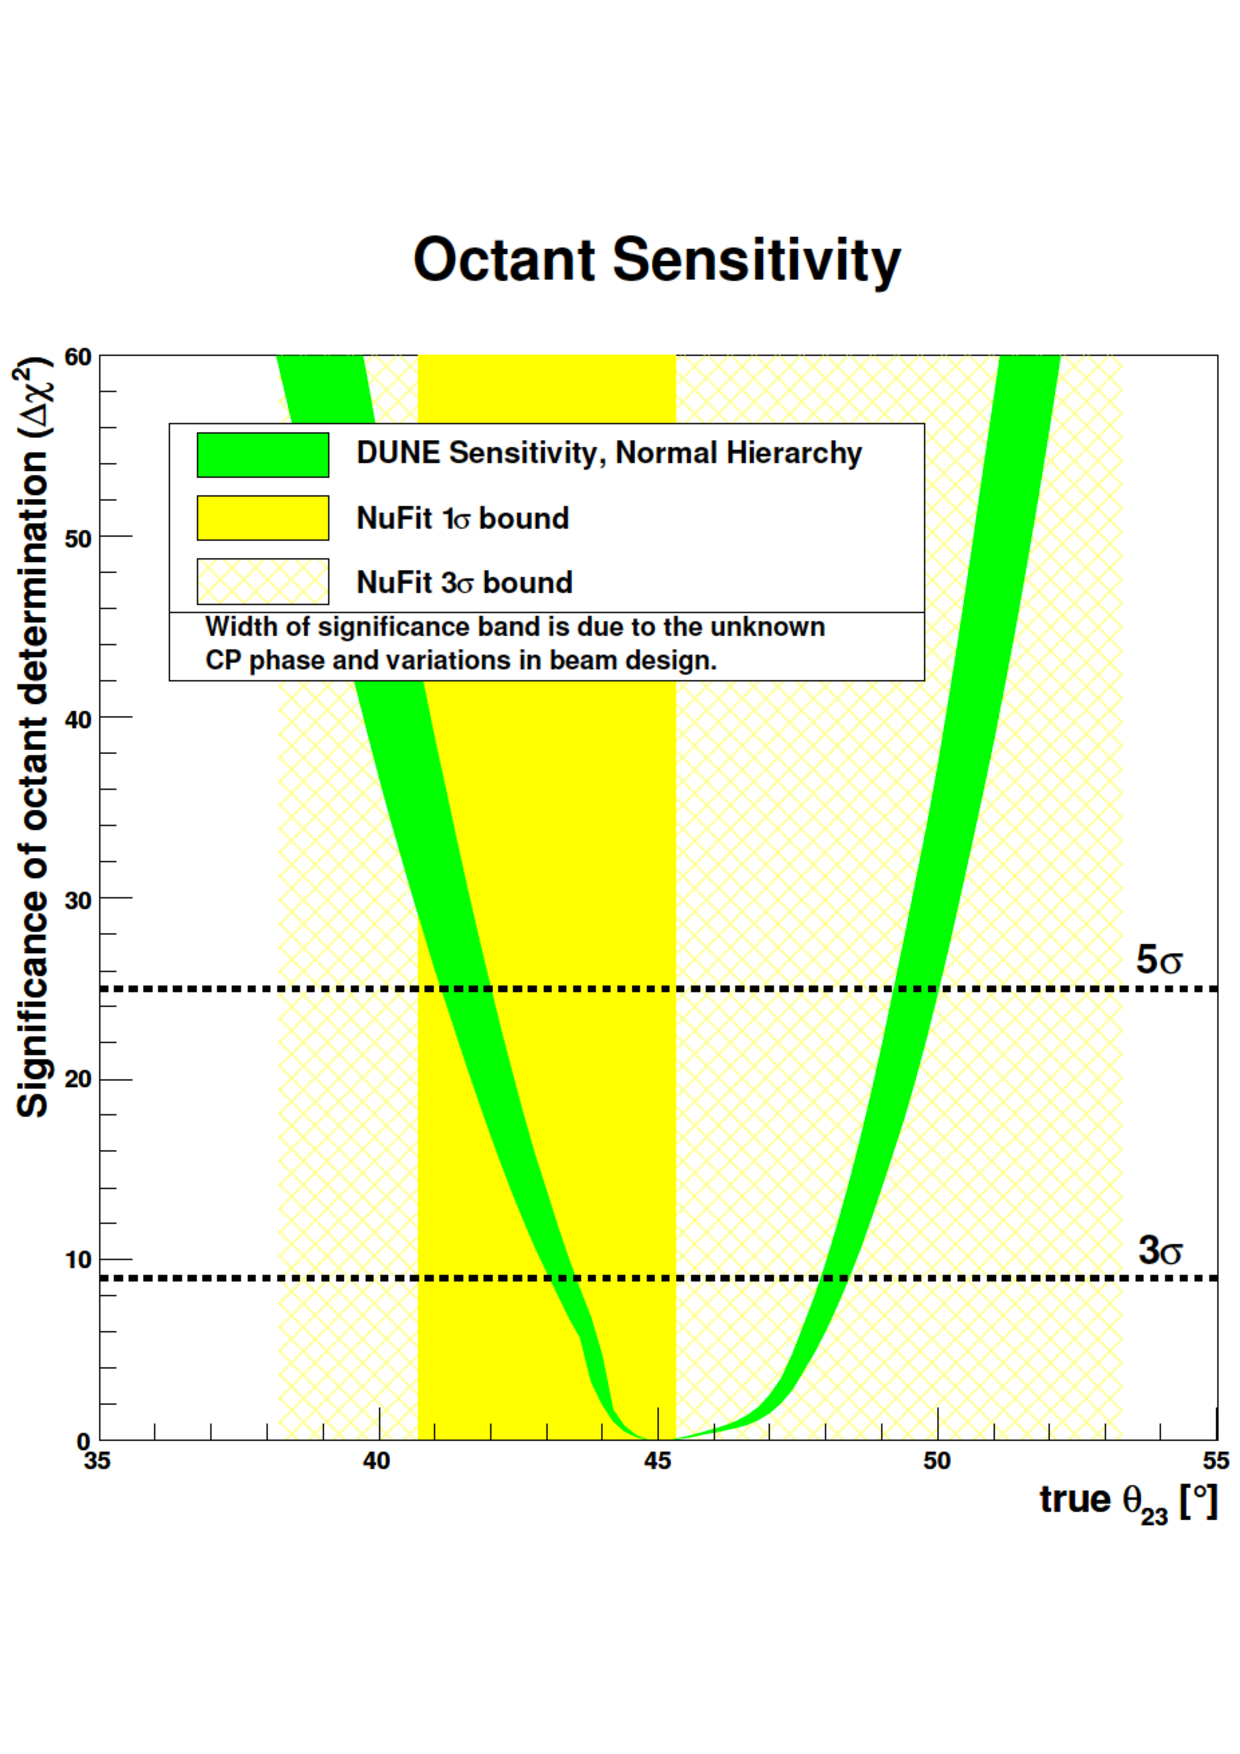
\includegraphics[width=0.5\textwidth]{DUNEOctantDetermination}
  \caption[The significance to which the octant of $\theta_{23}$ can be determined, for values of $\theta_{23}$]
          {The significance to which the octant of $\theta_{23}$ can be determined, for values of $\theta_{23}$. An exposure offering a 3$\sigma$ determination of the value of $\delta_{CP}$ for 75\% of the values of $\delta_{CP}$ is assumed. The green band shows the effect of different values of $\delta_{CP}$ and beam configurations. The yellow region show the 1$\sigma$ and 3$\sigma$ at the time of writing. The figure is taken from~\citep{DUNECDR_V2}.}
  \label{fig:DUNEOctantDetermination}
\end{figure}

The precision with which the values for $\sin^{2}\theta_{13}$, $\sin^{2}\theta_{23}$, and $\Delta m^{2}_{31}$ can be measured by DUNE are shown in Figures~\ref{fig:DUNETheta13Res},~\ref{fig:DUNETheta23Res}, and~\ref{fig:DUNEDeltaMRes} respectively. 

\begin{figure}[h!]
  \centering
  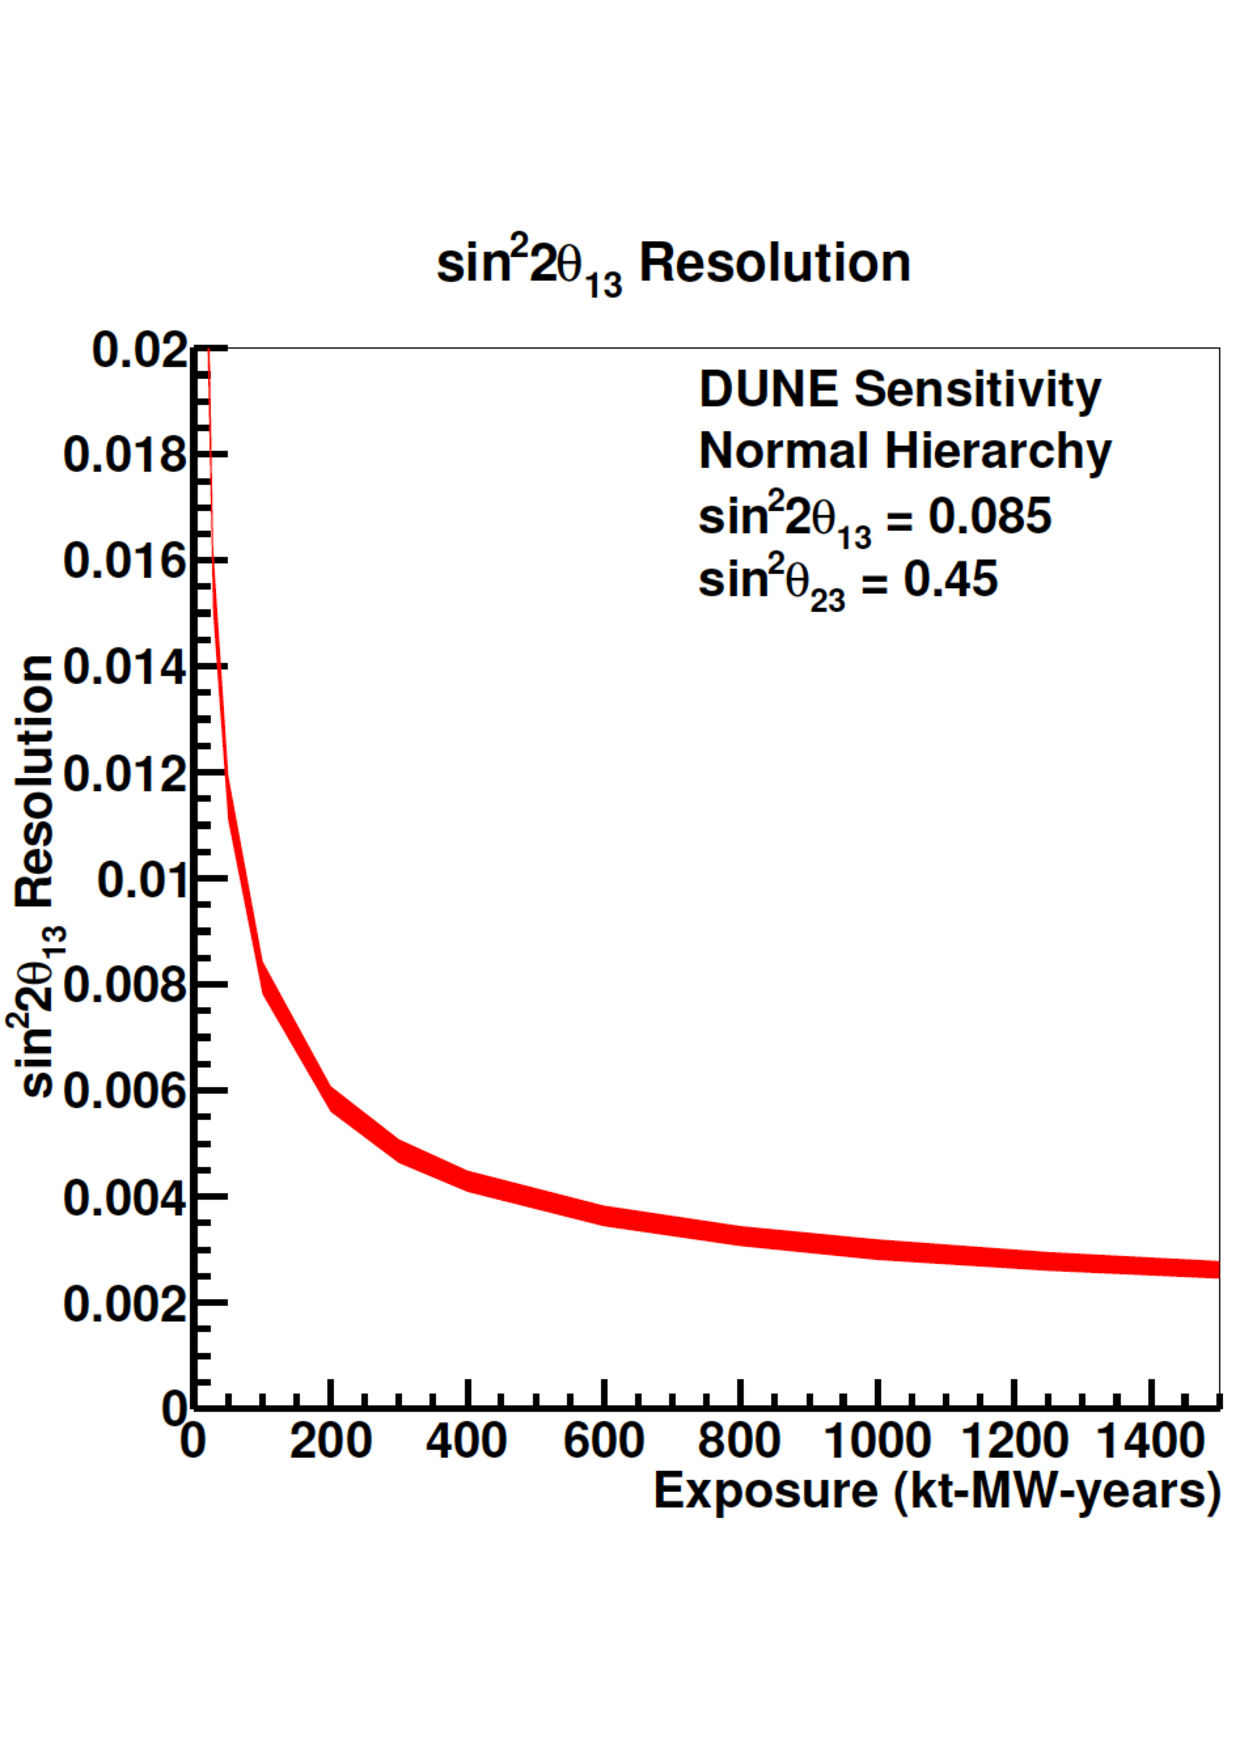
\includegraphics[width=0.5\textwidth]{DUNETheta13Res}
  \caption[The resolution with which DUNE will be able to determine the value of $\sin^{2}\theta_{13}$ for increasing exposures]
          {The resolution with which DUNE will be able to determine the value of $\sin^{2}\theta_{13}$ for increasing exposures. A normal hierarchy is assumed, and the bands show the sensitivities to the potential beam designs. The figure is taken from~\citep{DUNECDR_V2}.}
  \label{fig:DUNETheta13Res}
\end{figure}

\begin{figure}[h!]
  \centering
  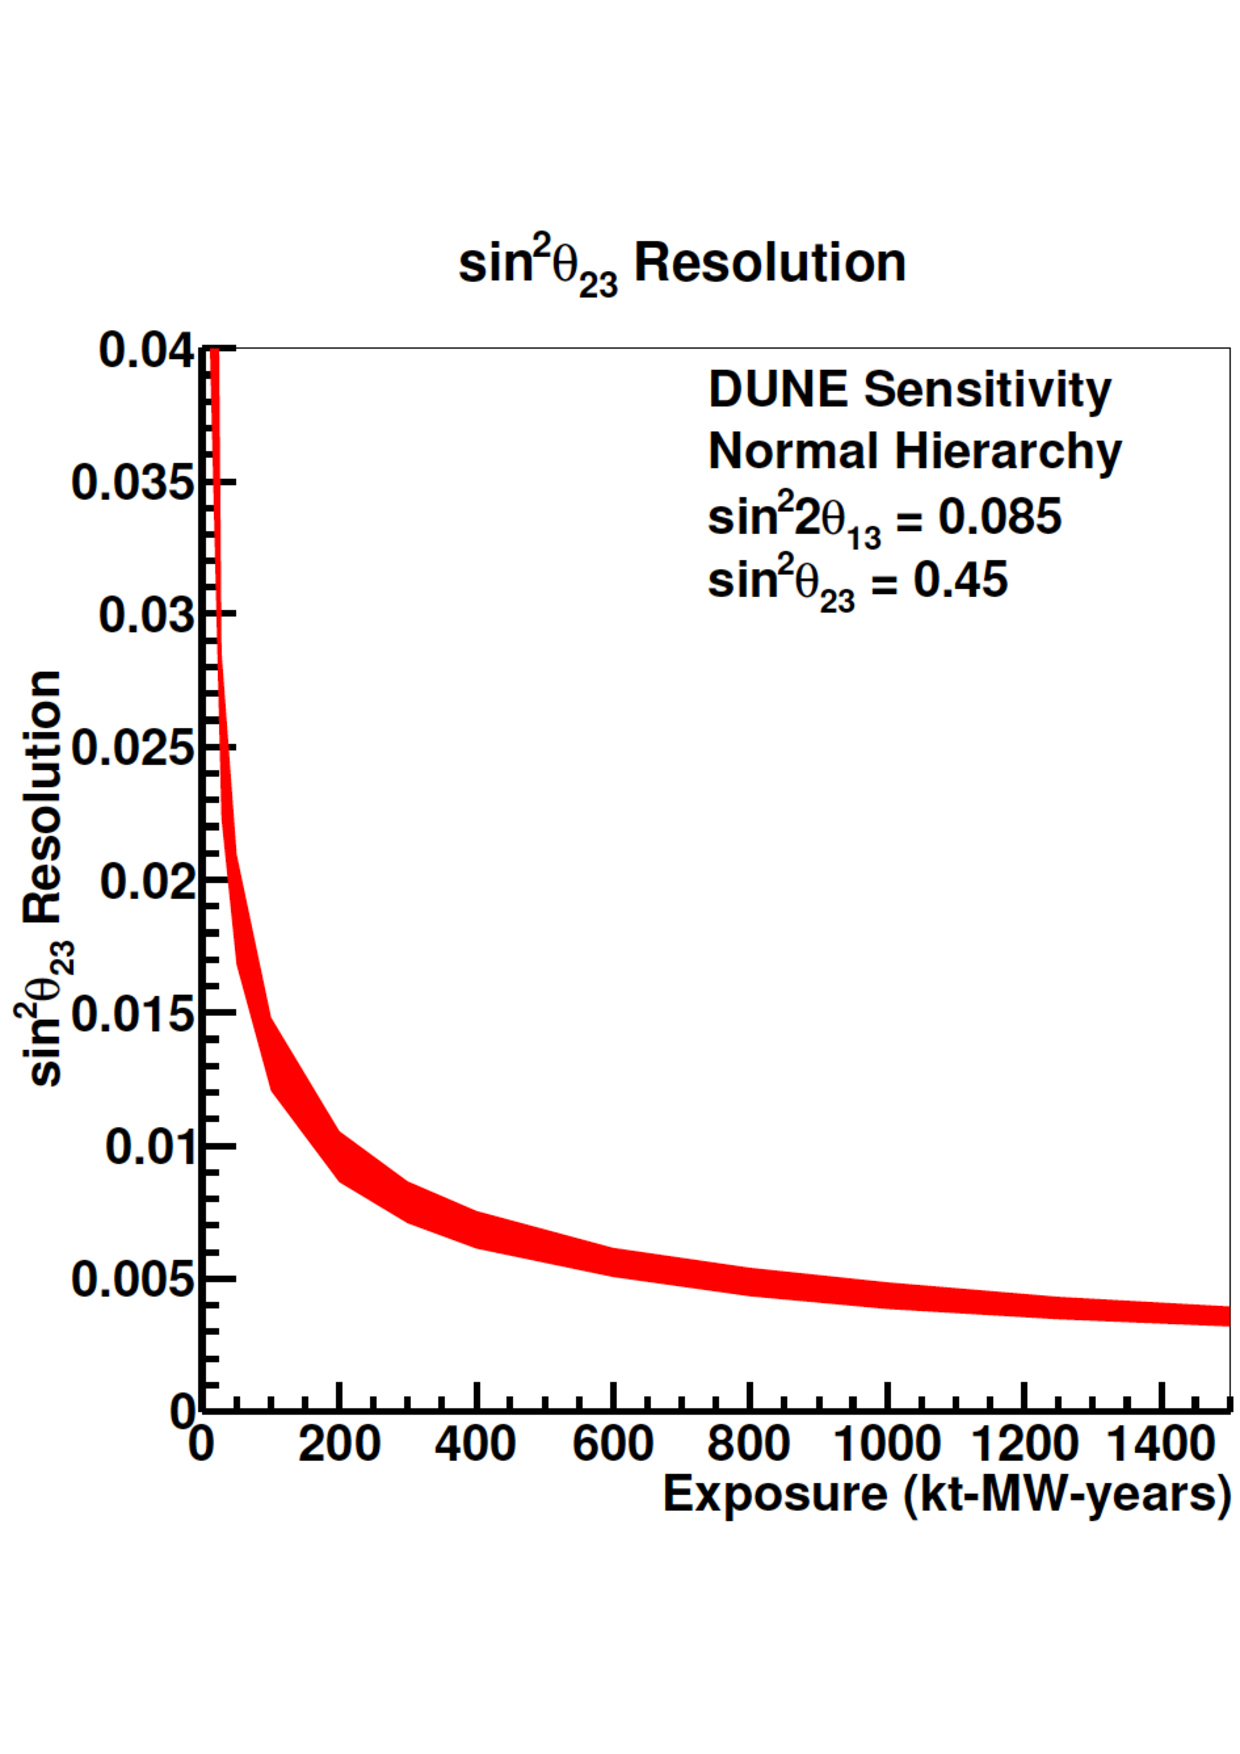
\includegraphics[width=0.5\textwidth]{DUNETheta23Res}
  \caption[The resolution with which DUNE will be able to determine the value of $\sin^{2}\theta_{23}$ for increasing exposures]
          {The resolution with which DUNE will be able to determine the value of $\sin^{2}\theta_{23}$ for increasing exposures. A normal hierarchy is assumed, and the bands show the sensitivities to the potential beam designs. The figure is taken from~\citep{DUNECDR_V2}.}
  \label{fig:DUNETheta23Res}
\end{figure}

\begin{figure}[h!]
  \centering
  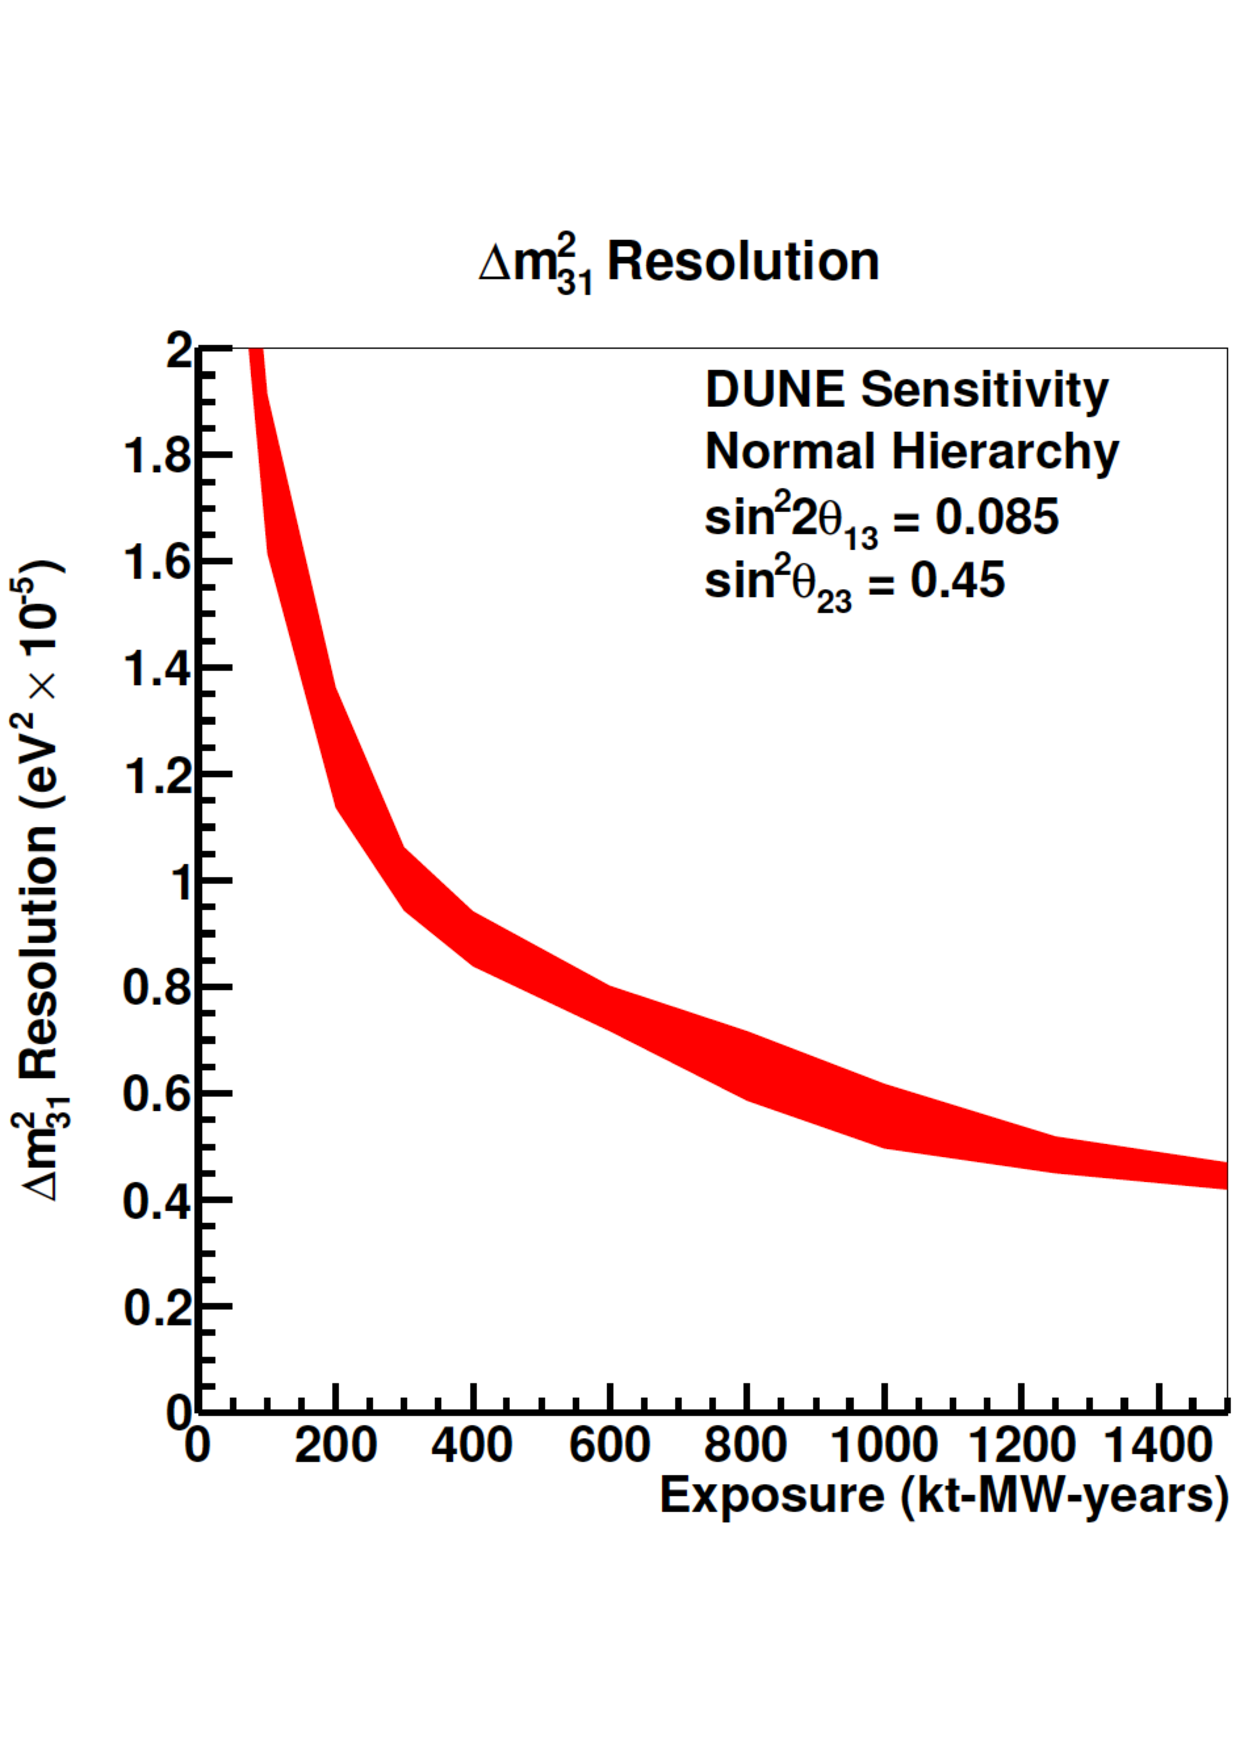
\includegraphics[width=0.5\textwidth]{DUNEDeltaMRes}
  \caption[The resolution with which DUNE will be able to determine the value of $\Delta m^{2}_{31}$ for increasing exposures]
          {The resolution with which DUNE will be able to determine the value of $\Delta m^{2}_{31}$ for increasing exposures. A normal hierarchy is assumed, and the bands show the sensitivities to the potential beam designs. The figure is taken from~\citep{DUNECDR_V2}.}
  \label{fig:DUNEDeltaMRes}
\end{figure}


%********************************** % 3.2 Section  *************************************
\subsection{Nucleon decay} \label{sec:DUNE_NDK}%Section - X.2.2

\begin{table}[h!]
\caption[Nucleon decay limits in DUNE and Super-Kamiokande]
        {Nucleon decay limits in DUNE and Super-Kamiokande, in some favoured decay channels.}
\centering
\label{tab:NDKLim}
\begin{tabular}{c c c c}
\toprule
{Total flux (cm$^{-2}$ s$^{-1}$)} & {Mean E$_{\mu}$ (GeV)} & {Mean slant depth (m w.e)} & {Mean $\theta$ ($^{\circ}$)} \\ 
\midrule
5.66 $\times$ 10$^{-9}$           & 283                    & 4532                       & 26                           \\
\bottomrule
\end{tabular}
\end{table}

%********************************** % 3.3 Section  *************************************
\subsection{Background to nucleon decay} \label{sec:BkNDK}  %Section - X.2.3

\begin{figure}[h!]
  \centering
  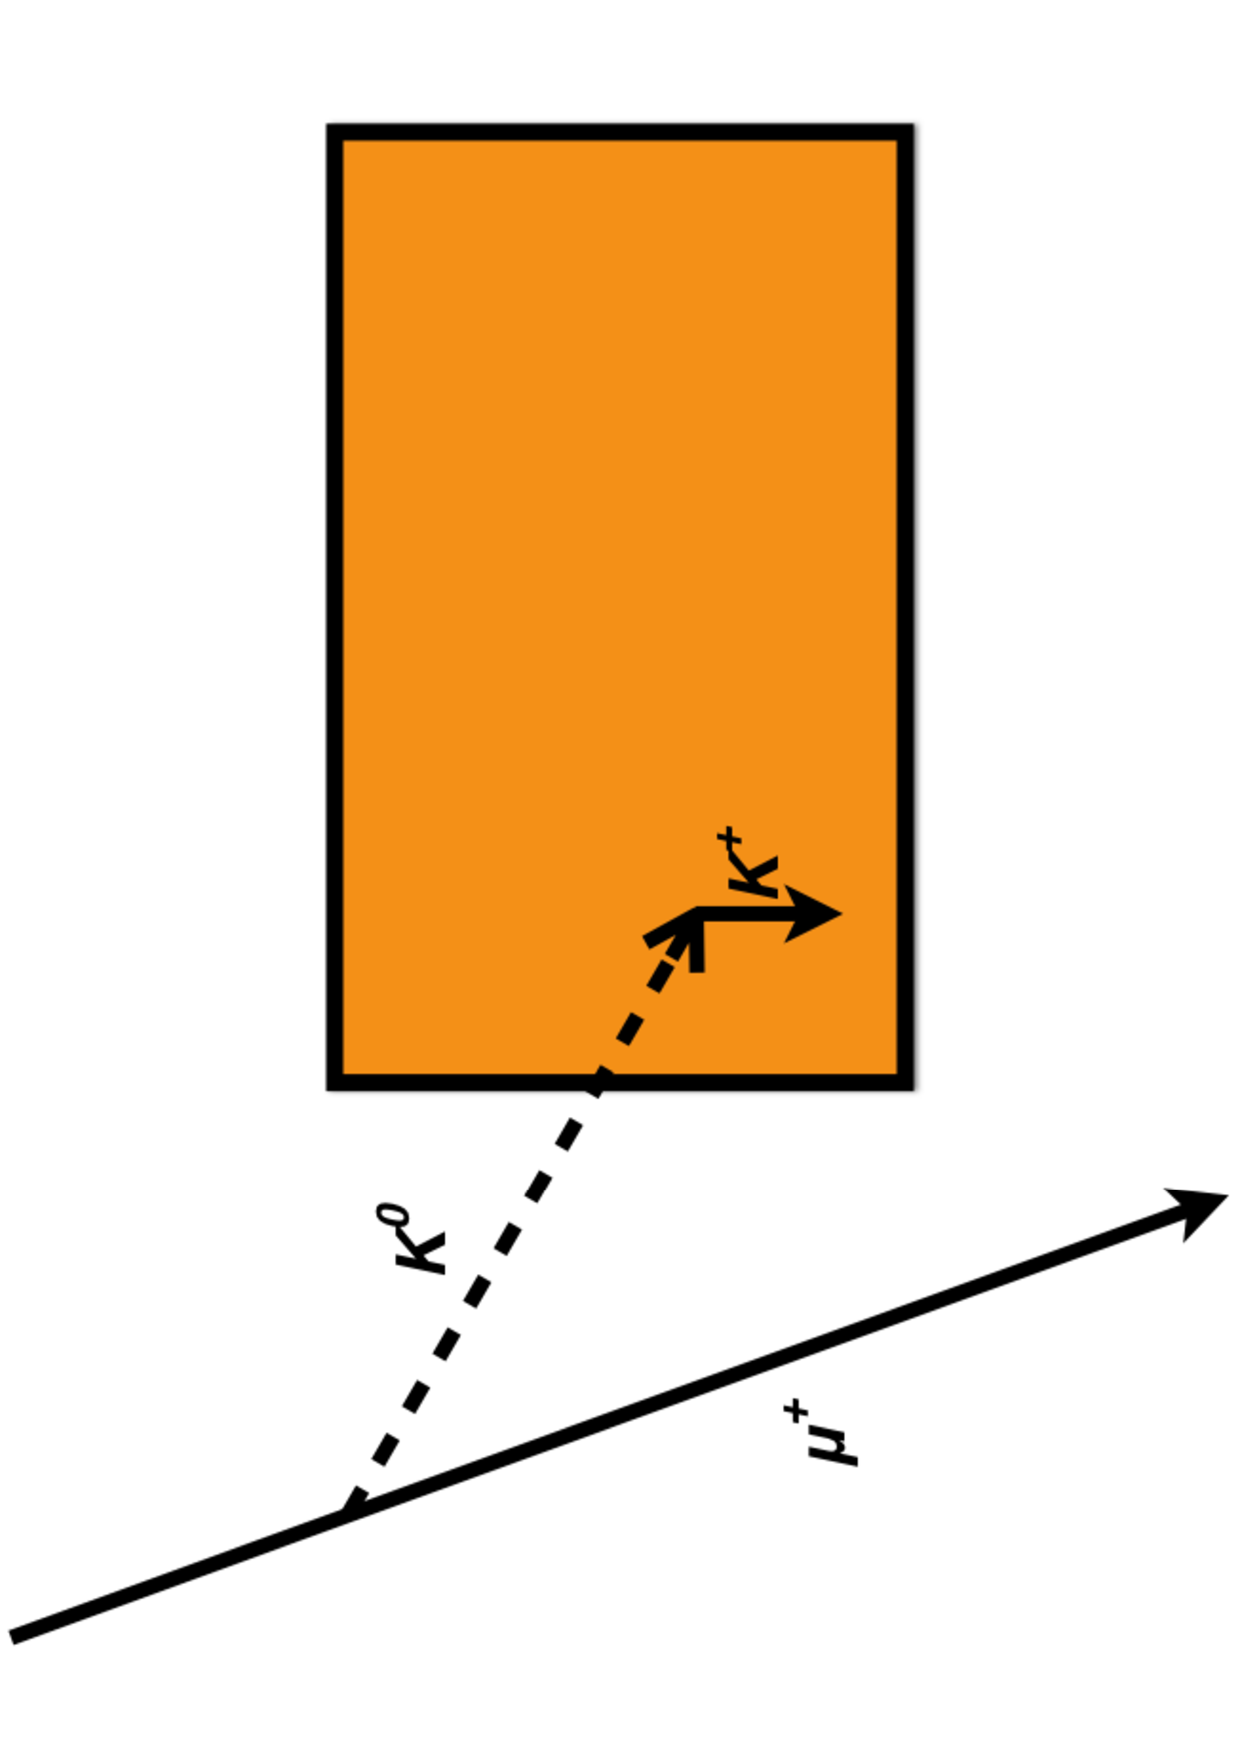
\includegraphics[width=0.5\textwidth]{KaonNDKInteraction}
  \caption[How the interaction of a cosmic muon can mimic a nucleon decay signature]
          {How the interaction of a cosmic muon can mimic a nucleon decay signature, by producing a $K^{0}_{L}$ which interacts far from the detector wall, producing an isolated kaon.}
  \label{fig:K0LongBackground}
\end{figure}

\subsection{Other physics opportunities} \label{sec:DUNE_Other}%Section - X.2.2

%********************************** %Second Section  *************************************
\section{The DUNE detectors and schedule} \label{sec:DUNEDetector} %Section - X.3

\subsection{The single phase detector design} \label{sec:DUNEDetector_SP}

\subsection{The dual phase detector design} \label{sec:DUNEDetector_DP}

\subsection{Potential near detector designs} \label{sec:DUNEDetector_Near}

%********************************** % Fourth Section  *************************************
\section{Path to building DUNE - The 35 ton prototype} \label{sec:The35tonDetector}  %Section - X.4

\begin{figure}[h!]
  \centering
  %\includegraphics[width=0.85\textwidth]{}
  \caption[The wrapped wires of the 35 ton]{A schematic showing what the wrapped wire planes of the DUNE detector designs looked like in the 35 ton.}
  \label{fig:35tonWireGeom}
\end{figure}

\begin{figure}[h!]
  \centering
  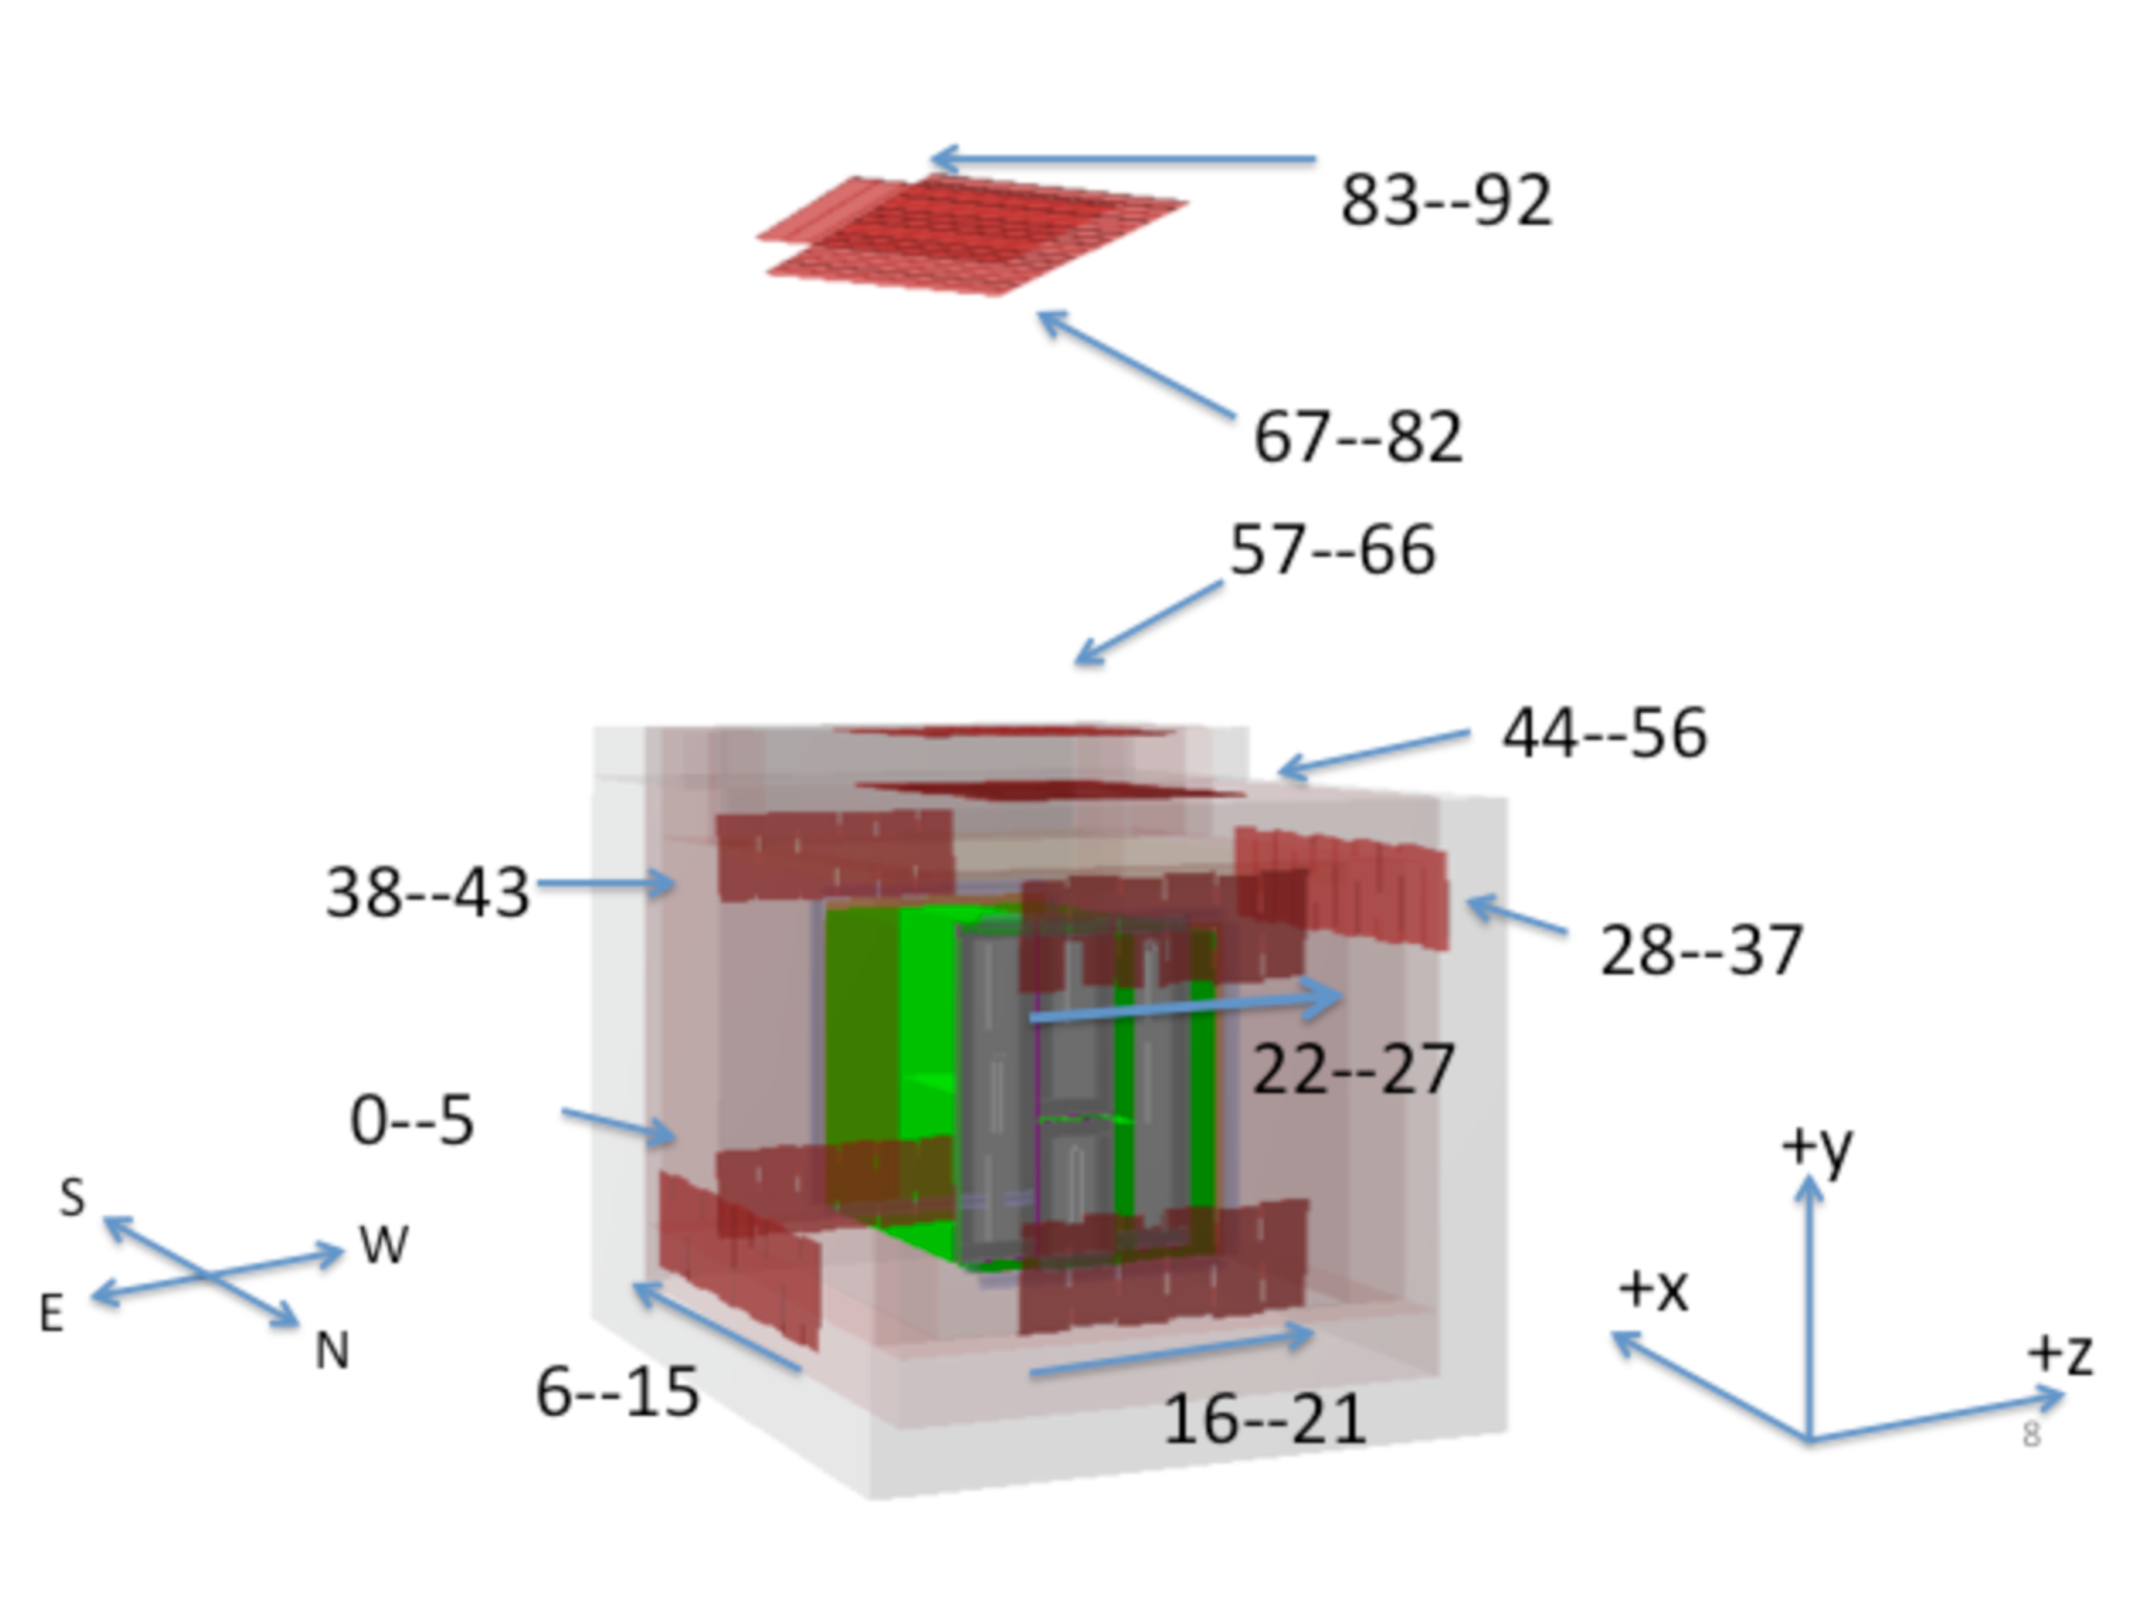
\includegraphics[width=0.85\textwidth]{35tonFullDetect}
  \caption[A representation of the counter locations in the 35 ton]
          {A representation of the counter locations in the 35 ton, with the magnetic and LArSoft co-ordinate systems shown. The other detector components can be seen inside the cryostat, such that the counters on the North wall are behind the short drift volume. The East - West counters are numbered 6-15 and 28-37 respectively. The North Lower - South Upper counters are numbered 16-21 and 38 - 43 respectively. The North Upper - South Lower counters are numbered 22-27 and 0-5 respectively. The telescope triggers are numbered 44-92 and are split into four groups.}
  \label{fig:35tonCounterLoc}
\end{figure}

%********************************** % Fifth Section  *************************************
\section{The DUNE software} \label{sec:LArSoft} %Section - X.5
The software package used by DUNE is called LArSoft~\citep{Church_LArSoft}~\citep{LArSoftOrg} which is a simulation, reconstruction and analysis package for Liquid Argon Time Projection Chamber (LArTPC) that is being used by many experiments in the US neutrino program. LArSoft has been developed to be detector agnostic, meaning that much of the code is shared between experiments. To this end it is envisioned that it will be used as a platform for constant development in existing experiments and those still in the planning phases such as DUNE. LArSoft is built around the Fermilab-supported \emph{analysis reconstruction framework} (\emph{art}). External packages such as ROOT~\citep{ROOT} and GEANT4~\citep{GEANT4} are incorporated into LArSoft meaning that the user does not have to coordinate specific versions of the packages as the newest versions are automatically incorporated. \\

There are numerous mechanisms by which particles can be generated within the software with external packages. One such package is GENIE~\citep{GENIE} which is used to study neutrino interactions and nucleon decays. Another package, Nuance~\citep{Nuance}, is a neutrino interaction generator specifically for Liquid Argon (LAr). Finally, CRY~\citep{CRY,CRY2} and CORSIKA!!!citep{CORSIKA} are cosmic ray events generators which are used to simulate the expected event rates for surface detector locations in absence of a neutrino beam. Recently the MUon Simulations UNderground (MUSUN)~\citep{MUSUN}~\citep{MUSUN2} generator which takes the output of MUon SImulation Code (MUSIC)~\citep{MUSUN}~\citep{MUSIC}~\citep{MUSIC2} has also been incorporated, see Section~\ref{sec:FDIncorporation} for further details. It is also possible to use an inbuilt single particle generation mode which is fully tuneable as particle type, momenta, positions and directions can all be varied. \\

The co-ordinates and angles in LArSoft are defined as follows, and schematic representations of how this appears in the 35 ton are shown in Figure~\ref{fig:LArSoft_coords}:
\begin{itemize}
\item $x$ - The beam direction, with maximal $x$ being where the beam enters the detector.
  \begin{itemize}
  \item In the 35 ton prototype where there is no beam positive $x$ is in the opposite direction to that which electrons drift in the large TPC, where $x$ = 0 is the position of the APA frames in the long drift volume.
  \item In the far detector geometry $x$ = 0 is defined as the midpoint between the two rows of CPAs 
  \end{itemize}
\item $y$ - The vertical direction, with maximal $y$ being the most highest point.
  \begin{itemize}
  \item In the 35 ton $y$ = 0 is halfway between the gap created by the two centre APAs which are mounted one above the other.
  \item In the far detector $y$ = 0 is defined as the midpoint between the two vertical layers of TPCs.
  \end {itemize}
\item $z$ - Defined as such to have a right handed co-ordinate system.
  \begin{itemize}
  \item In the 35 ton $z$ = 0 is at the edge of the leftmost APA frame when looking down the long drift volume.
  \item In the far detector $z$ = 0 is defined at the edge of the leftmost APA frame when looking down the long drift volume.
  \end{itemize}
\item $\theta$ - The angle that a vector makes from the $x$ axis in the $xy$ plane.
\item $\phi$ - The angle between the $z$ axis and the vector.
\end{itemize}

\begin{figure}[h!]
  \centering
  \begin{subfigure}{0.45\textwidth}
    \centering
    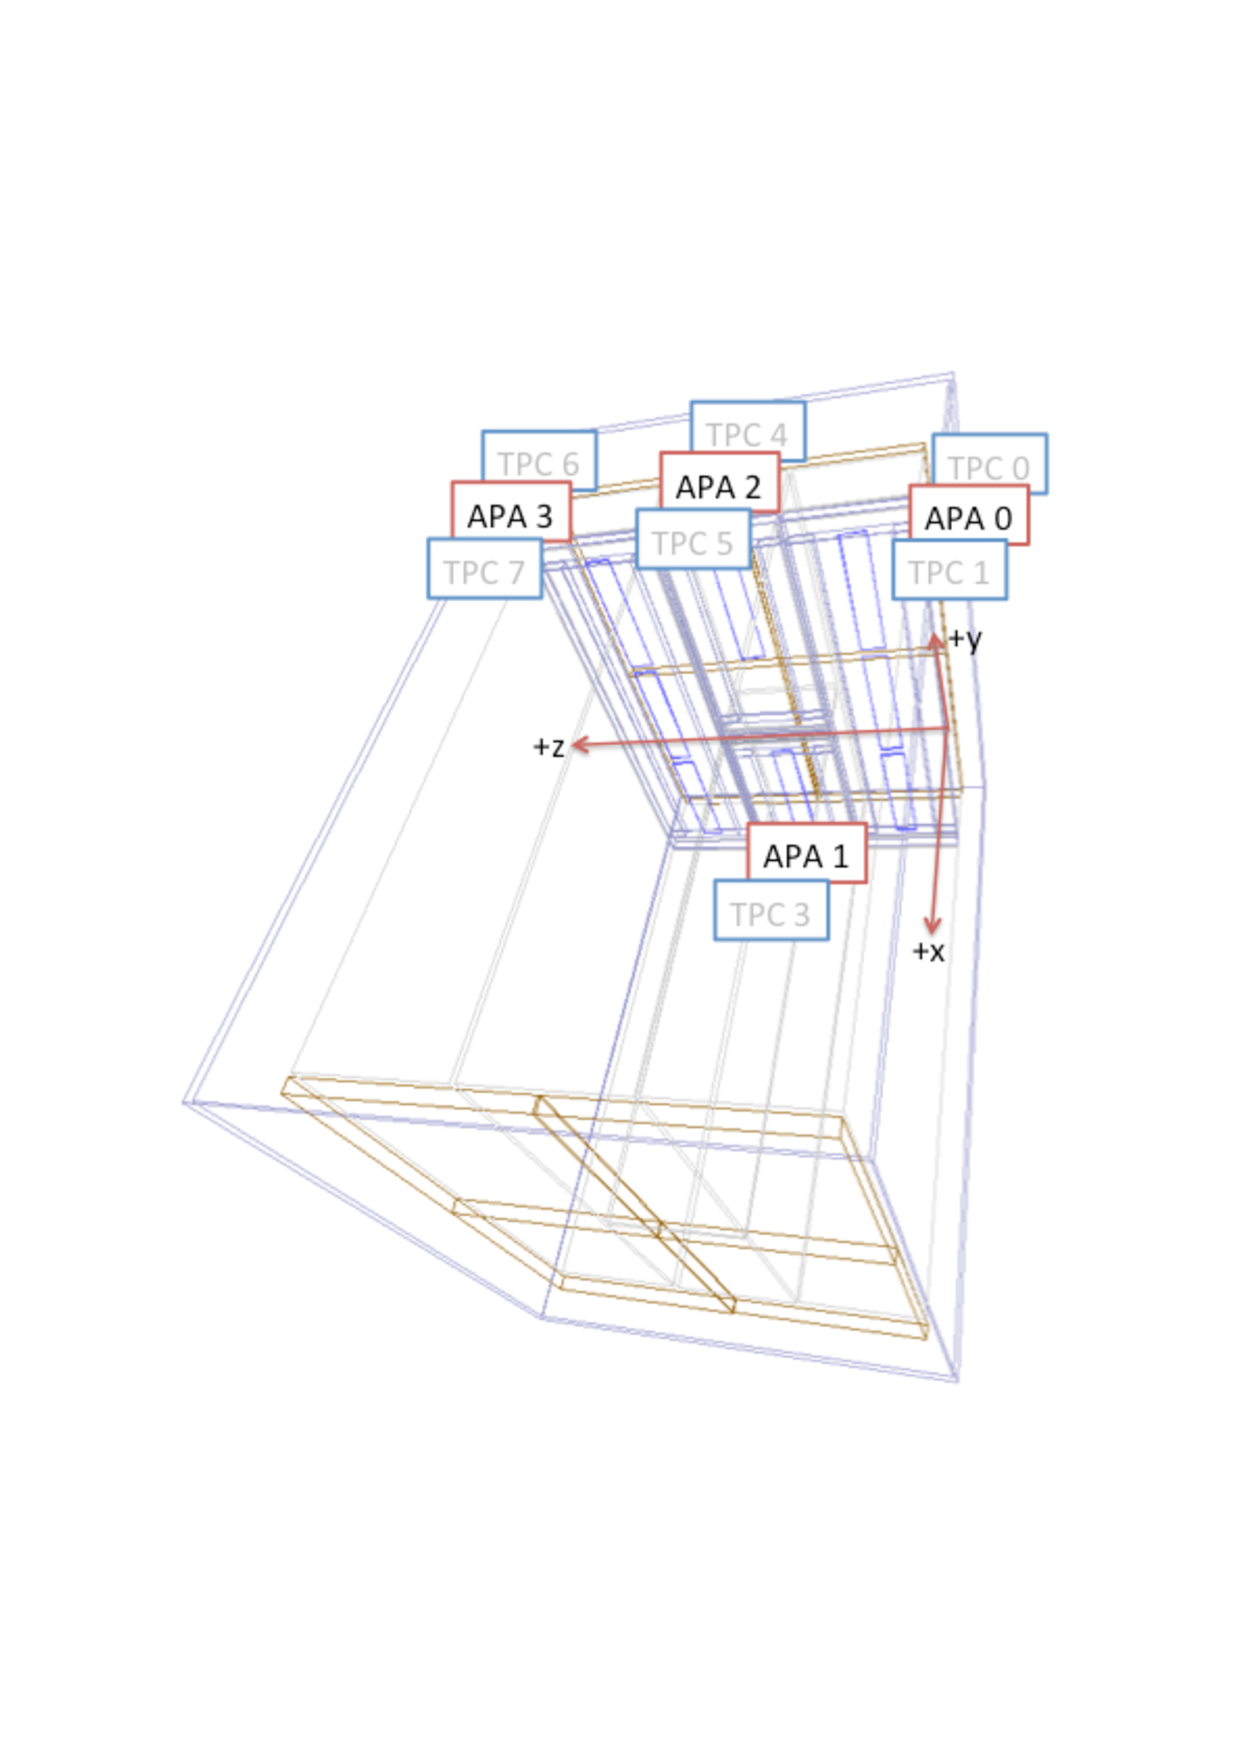
\includegraphics[width=\textwidth]{35ton_APASchem}
    \caption{The location of the origin of the 35 ton co-ordinate system in 3D.}
  \end{subfigure}
  \hspace{0.08\textwidth}
  \begin{subfigure}{0.45\textwidth}
    \centering
    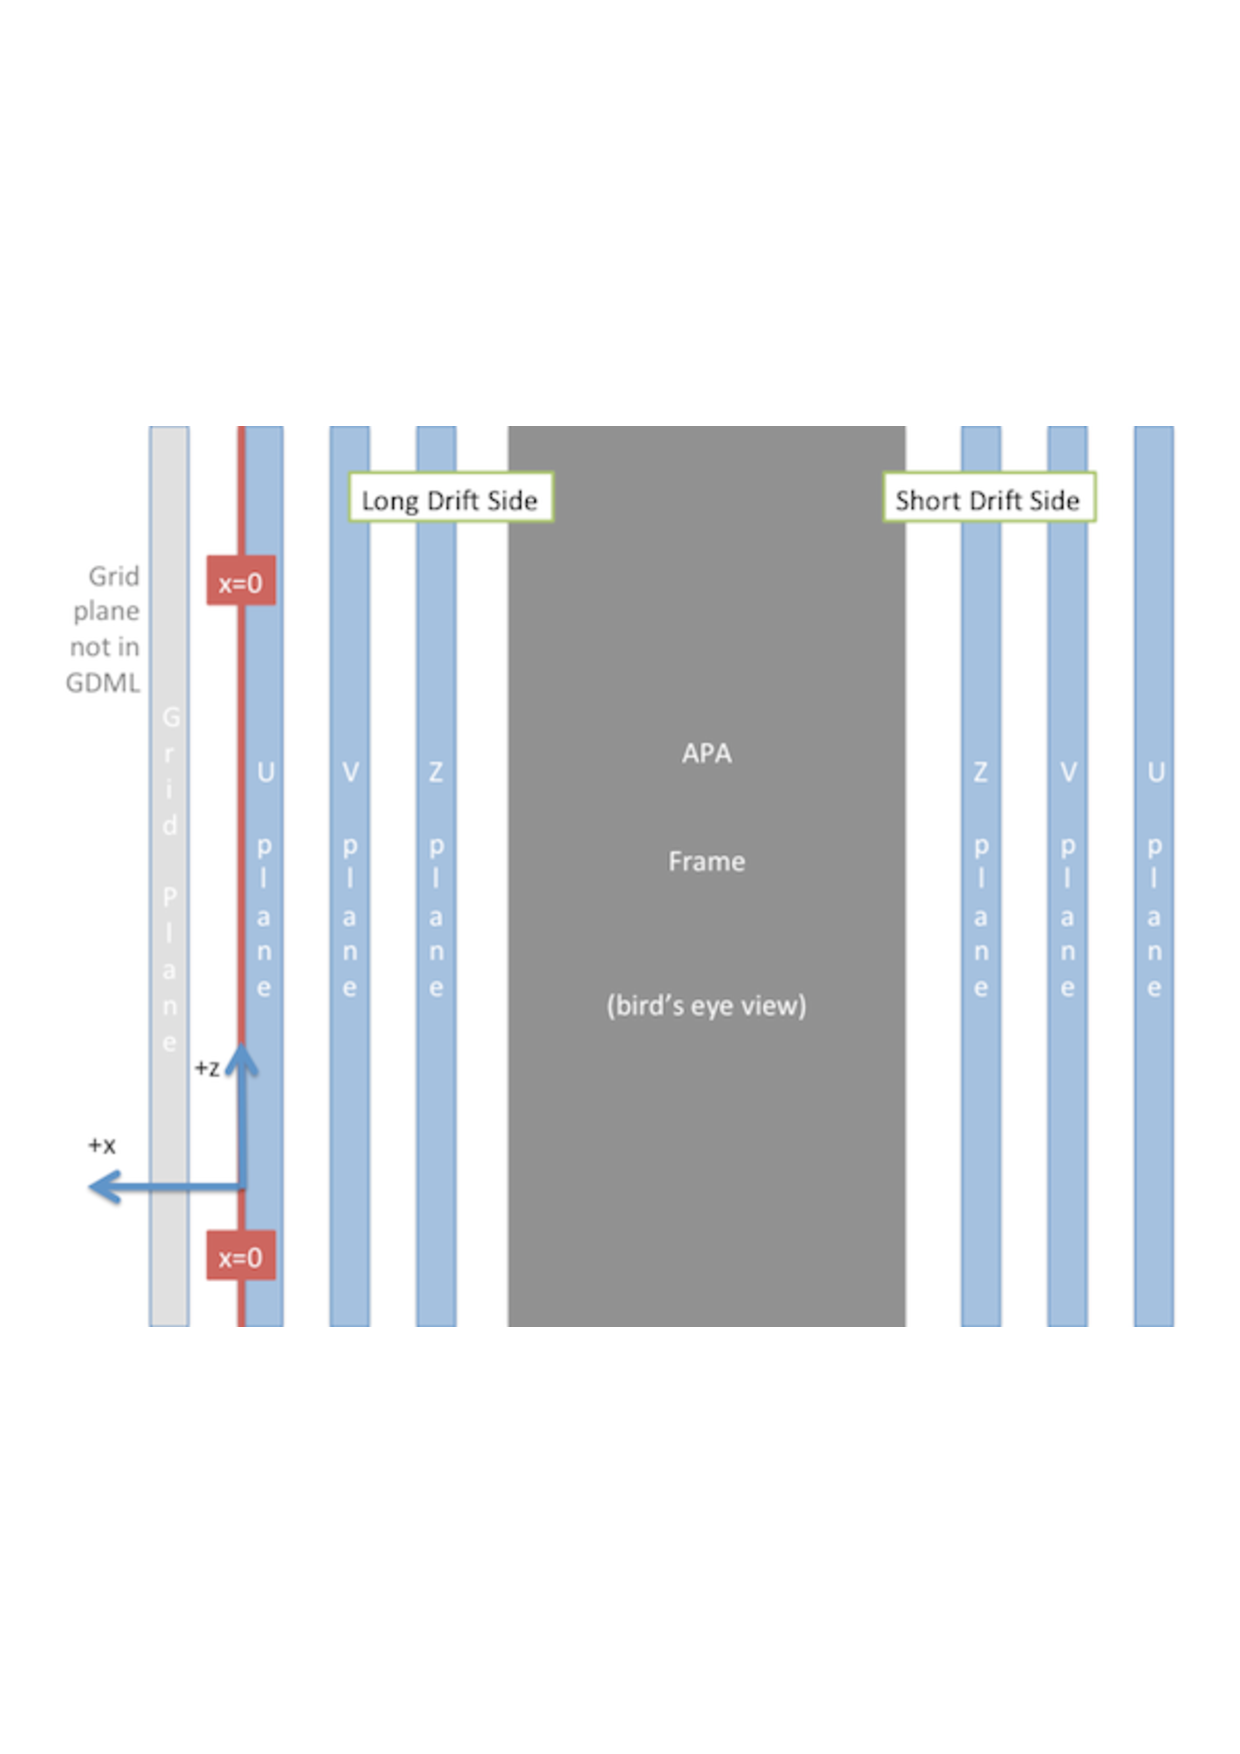
\includegraphics[width=\textwidth]{35ton_xCenter}
    \caption{The location of the origin of the 35 ton co-ordinate system in a 2D aerial view.}
  \end{subfigure}
  \caption[The LArSoft co-ordinate system as it is represented in the 35 ton.]
          {The LArSoft co-ordinate system as it is represented in the 35 ton. Left shows the location of the origin relative to the TPC detector components. The four APAs, and eight TPCs are shown, where the even numbered TPCs are on the short drift side, $\sim$20 cm drift, and the odd numbered TPCs are on the long drift side, $\sim$250 cm drift. The CPAs are also shown as the objects with a brown outline. Right shows the location of the origin with respect to the APAs. The wire planes are shown, the U and V planes are induction wires, whilst the Z planes are collection wires.}
  \label{fig:LArSoft_coords}
\end{figure}

The simulation of particles is usually split into five separate distinct processes to reflect the different stages in which development often progresses. The advantage of segmenting the computational process in this way is that improvements can easily applied to a file without rerunning the entire chain. This is especially important when large Monte Carlo or data samples are produced for general use within collaborations so that users are able to concentrate on improving a specific part of the computational process. When these all-purpose samples are produced the analysis performed provides users with any Monte Carlo truth information along with the reconstructed quantities for use in analyses performed outside LArSoft. The computational process is often broken down in the following way:
\begin{itemize}
\item Particle generator.
\item Particle transport using GEANT4.
\item Full detector simulation, including detector responses. 
\item Full event reconstruction.
\item Analysis.
\end{itemize}

Later significant focus will be given to the reconstruction of TPC data, and so it is necessary to briefly illustrate the mechanisms by which TPC data is reconstructed in LArSoft. Much of the information presented below is summarised in~\citep{LArSoftRecoNote}~\citep{LArSoftOrg}. After the full detector simulation or data taking, detector effects such as the electronics response function and a pedestal offset have to removed. Once these effects are removed the signal is estimated using the optimal value of $signal/noise$ which would produce the measured signal. This process, called deconvolution, does not conserve pulse height and is not guaranteed to preserve the normalisation. The deconvoluted signals are all unipolar distributions which means that Gaussian distributions can then be fitted to them when trying to reconstruct hits. This is shown in Figure~\ref{fig:LotsOfHits}, and explained further below.\\

\begin{figure}[h!]
  \centering
  \begin{subfigure}{0.95\textwidth}
    \centering
    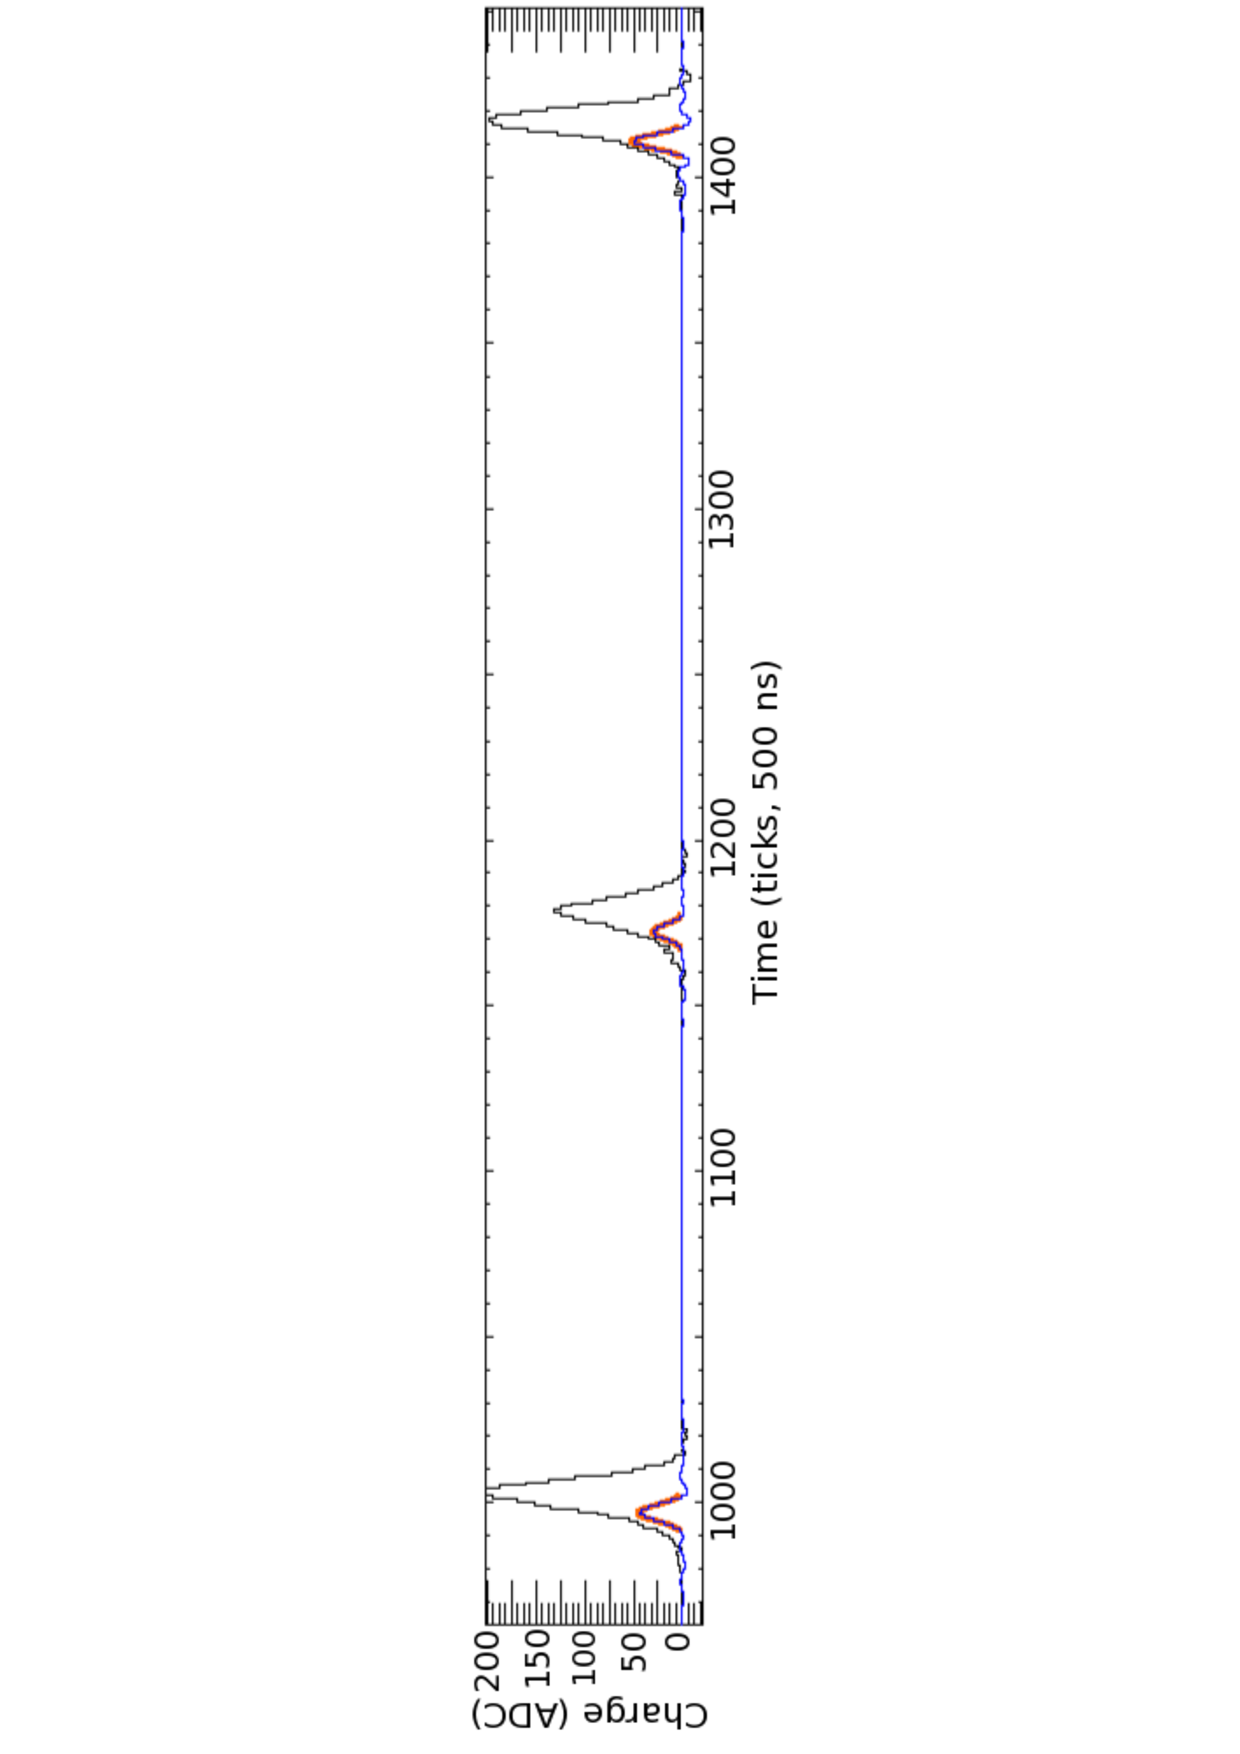
\includegraphics[width=\textwidth]{CollectionPlane}
    \caption{Collection plane depositions.}
    \label{fig:LotsOfHits_Col}
  \end{subfigure}
  \begin{subfigure}{0.95\textwidth}
    \centering
    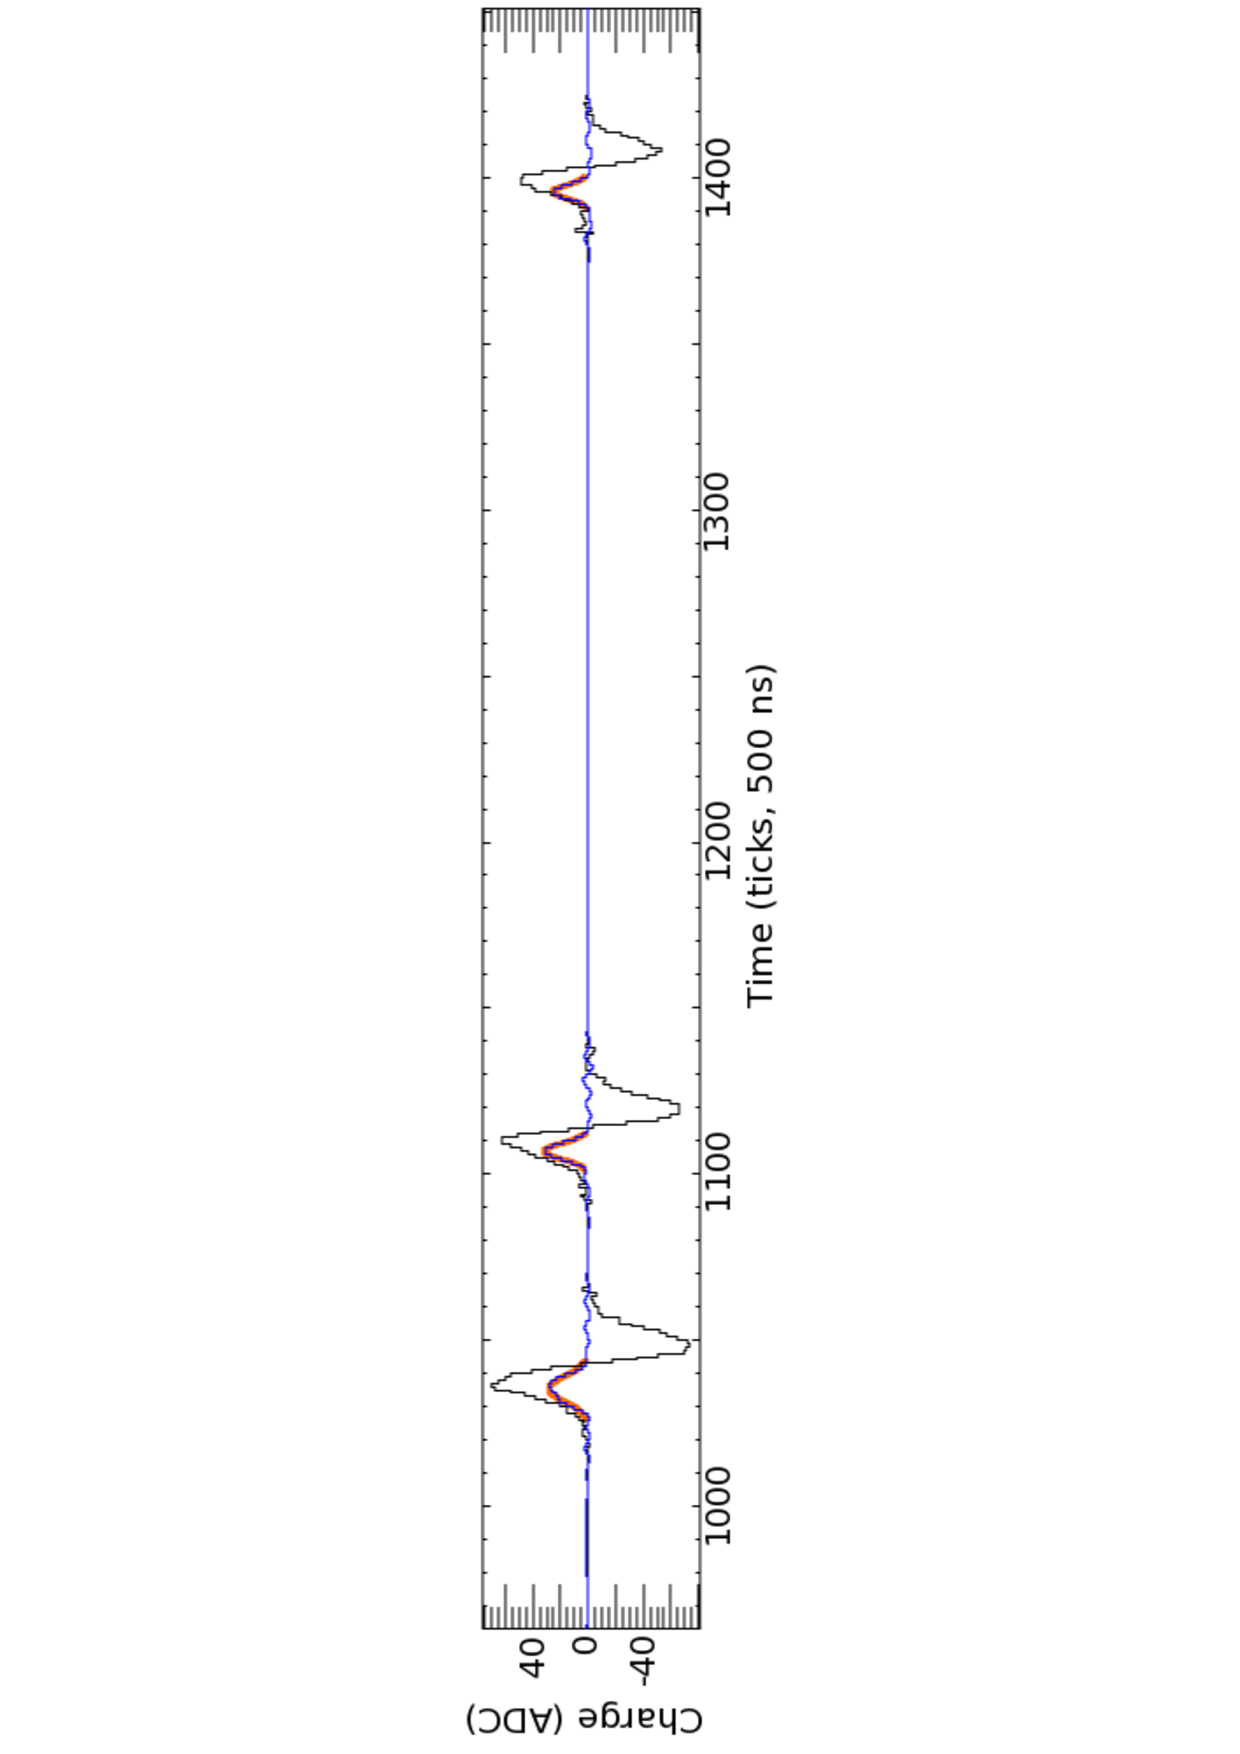
\includegraphics[width=\textwidth]{InductionPlane}
    \caption{Induction plane depositions.}
    \label{fig:LotsOfHits_Ind}
  \end{subfigure}
  \begin{subfigure}{0.95\textwidth}
    \centering
    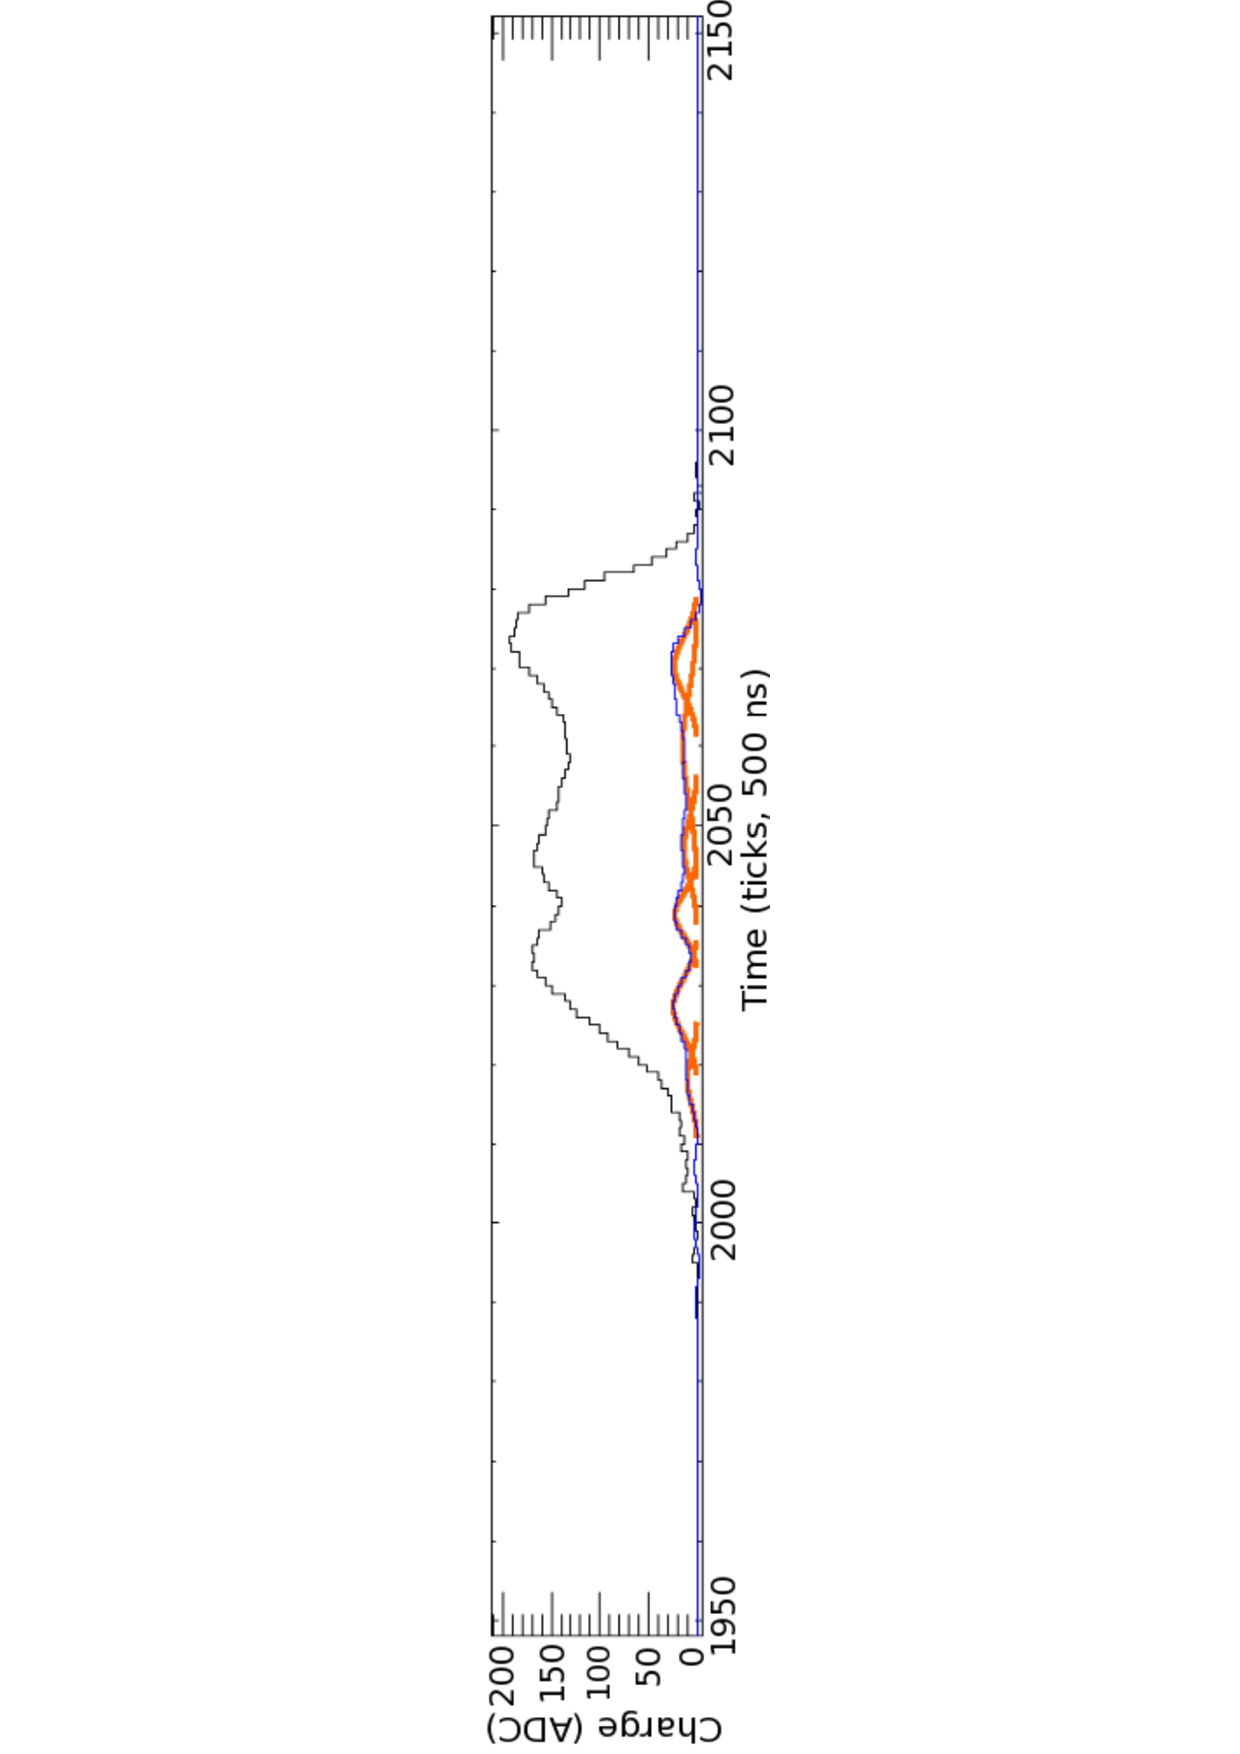
\includegraphics[width=\textwidth]{Complex}
    \caption{A large collection plane deposition over a large period of time.}
    \label{fig:LotsOfHits_Big}
  \end{subfigure}
  \caption[Reconstructed hits from simulated energy depositions]
          {The raw and deconvoluted signals with reconstructed hits on single wires for simulated energy depositions. The depositions, from particles generated by CRY, are not from a single event and have been selected for demonstration purposes only. The plots are shown with increasing charge (ADC) on the $y$ axis, and increasing time (ticks, 500 ns) on the $x$ axis. The black lines represent the raw signals, the blue lines represent the deconvoluted signals and the orange lines represent the reconstructed hits. Top shows depositions on a collection plane wire, it can be seen that the raw signal is unipolar. Middle shows depositions on an induction plane wire, it can be seen that the raw signal is bi-polar whilst the deconvoluted signal and reconstructed hits are unipolar. Bottom shows a complex deposition on a collection plane wire, where multiple reconstructed hits are required to reproduce the deconvoluted signal.}
  \label{fig:LotsOfHits}
\end{figure}

The deconvoluted signals are reconstructed into hits by identifying regions that are above a threshold value and then attempting to replicate the signal in these regions by introducing Gaussian distributions. For isolated hits this is typically achieved using only one Gaussian distribution, however for large energy depositions over a large period time where many particles are involved, multiple Gaussian distributions are often required. Large energy depositions are also possible when the direction of the particle aligns with a wire, this means that all of the deposited energy is collected on this single wire. Examples of reconstructed hits are shown in Figure~\ref{fig:LotsOfHits}. These figures are taken from separate CRY simulated events, and so do not correspond to a continuous simulated event. They have been selected only as a demonstration of the process of hit reconstruction. Figures~\ref{fig:LotsOfHits_Col} and~\ref{fig:LotsOfHits_Ind} show multiple time-separated energy depositions on a collection and induction wire respectively. A more complex energy deposition on a collection plane wire is shown in Figure~\ref{fig:LotsOfHits_Big} where energy depositions from many particles at similar times have created a complicated energy deposition that requires many reconstructed hits to explain. \\

As noted in Section~\ref{sec:DUNEDetector} and Section~\ref{sec:The35tonDetector} the DUNE FD and the 35 ton both have wrapped wires on the induction planes. A result of this is that the location of the reconstructed hit on an induction wire is ambiguous as a single wire has many wire segments, as shown in Figure~\ref{fig:35tonWireGeom}. An important feature of this ambiguity is that the TPC in which the hit occurred cannot be identified unless it is combined with another hit. These ambiguities do not extend to the collection plane wires as they are not wrapped and so consist of only a single wire segment in a single TPC. Hits are combined across the three planes by identifying wire segments on each plane which intersect and have hits at common times. In the traditional reconstruction process only hits that make these so-called 'triple points' are considered disambiguated, with other hits being identified as noise hits causing them to be discarded. \\

The inclination of the wire planes has to be carefully chosen so as to minimise both the number of wires required and the number of times that wire triplets intersect. This is shown in Figure~\ref{fig:WirePitches}, where the wire inclinations used in the 35 ton detector, are compared to those in the DUNE FD reference design. The inclination of wires in the 35 ton was 45$^{\circ}$ $\pm$ 0.7$^{\circ}$ meaning that many wire triplets cross twice and some wire pairs cross three times. When wire triplets cross multiple times the triplet which has the smallest distance between the common intersection point and the two, two-wire intersection points, is chosen as the best intersection candidate. This is shown as the 'Good intersection' on the right panel in Figure~\ref{fig:WirePitches}. The different wire pitches are necessary so that one of the triple points can be evaluated to be a better candidate, as with a wire pitch of 45$^{\circ}$ it can be impossible to distinguish between different triple points. The inclination of wires in the FD was chosen to be 36$^{\circ}$ to remove the possibility of multiple intersection points, as given the geometry of the APAs multiple intersection points are impossible and so disambiguation is much simpler. The lower inclination results in more induction wires being required though, making it more expensive to instrument the detector. It is also important that all wires on a given APA are either read at the top or base of the APA, depending on whether the APA is at either the top or the base of the detector respectively. This is because there must be minimal space between TPCs in the DUNE FD to reduce the internal dead space, and so TPCs cannot be read out along the sides as this would require a non-negligible amount of space to accommodate the cabling.\\

\begin{figure}[h!]
  \centering
  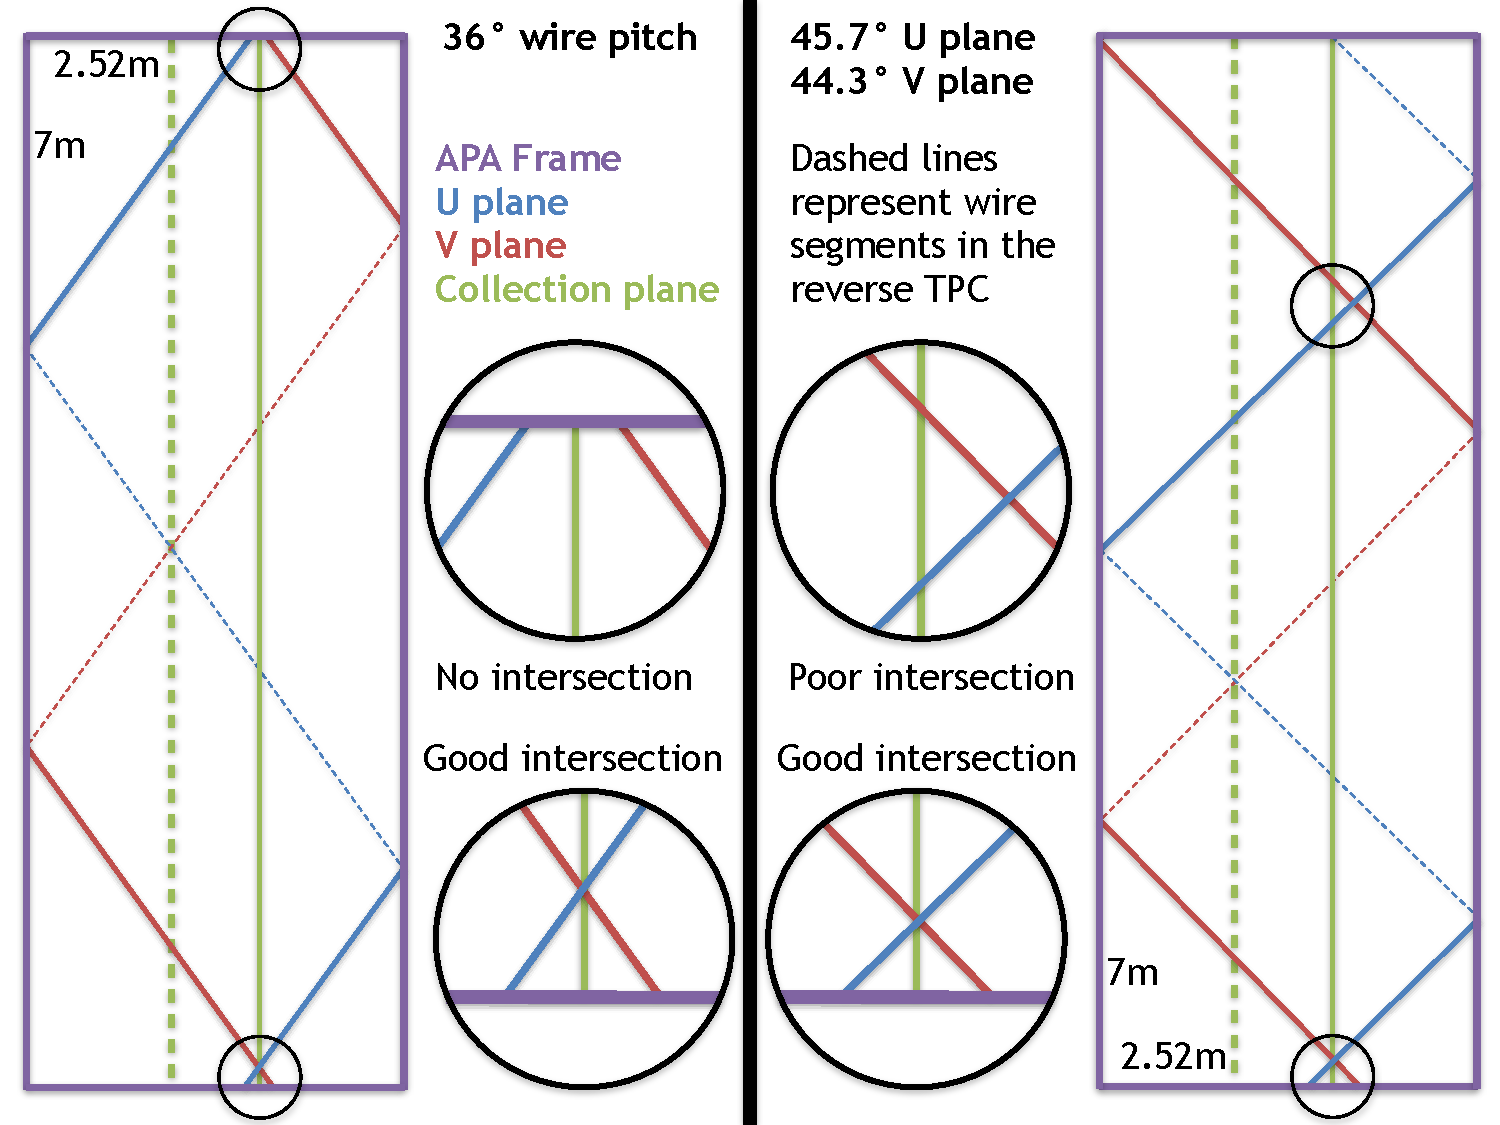
\includegraphics[width=0.85\textwidth]{WireAngleCondition}
  \caption[Performing disambiguation with different wire pitches.]
          {The effect that different wire pitches have on the ability to perform disambiguation in APAs with the far detector geometry. The left panel shows a wire pitch of 36$^{\circ}$, which is the reference design for the far detector, whilst the right panel shows wire pitches of 45$^{\circ}$ $\pm$ 0.7$^{\circ}$, as was used in the 35 ton. The left panel shows that only one 'triple point' can be made with the three wires shown, and so disambiguation is relatively trivial. The right panel shows that two 'triple points' can be made with the three wires shown, the 'triple point' where the three wires have a common intersection point is labelled as a 'good intersection' and it is this intersection point which would be chosen for the disambiguated hit.}
  \label{fig:WirePitches}
\end{figure}

Once the hits have been disambiguated they are combined to make clusters in each of the three planes, before the clusters are merged to make reconstructed tracks or showers. The clustering process is usually performed in wire-tick space on each plane separately, where all the hits from a single track or shower should be make a single cluster on each plane. It is possible to seed the start of clusters by using imaging techniques such as a Harris transform~\citep{HarrisTrans}, or to identify straight lines by using Hough transforms~\citep{HoughTrans}. As hits from a physical entity are unlikely to remain on a single channel or all come at identical times, clusters are often spread out over many channels for a range of times especially when performing clustering for showers. \\

Once clusters have been identified in each plane they can then be merged into 3-dimensional tracks and showers. The two most common tracking algorithms are PMTrack~\citep{PMTrack} and Pandora~\citep{Pandora}, and the most common showering algorithm is EMShower~\citep{EMShower}. Once 3D objects have been reconstructed, the calorimetric quantities need to be determined, this is often done separately for each plane. Two models exist for calculating $\frac{dE}{dx}$ in LArSoft, Birks model~\citep{BirksModel} and a modified Box model~\citep{PIDA_Paper} which uses a correction to the Box model~\citep{BoxModel} at low values of $\frac{dE}{dx}$. Normally the modified Box model is used as it holds for both large and small ionisation's, whereas Birks model experiences difficulties at large ionisation's and the traditional Box model struggles at low $\frac{dE}{dx}$. Both models incorporated in LArSoft, calculate the $\frac{dE}{dx}$ of a hit using the deposited charge ($dQ$) and the track pitch ($dx$) of the hit as well as the conversion of ADC value to number of electrons ($C_{GeV \rightarrow e^{-}}$), a correction due to electron lifetime ($C_{lifetime}$), the LAr density ($\rho$), the electric field ($E_{field}$) and the tuneable electron recombination factors ($Recomb_{X}$). The series of equations used in Birks model are shown in Equation~\ref{eq:Birks}, whilst those used in the modified Box model are shown in Equation~\ref{eq:ModBox}. \\

\begin{subequations}
  \label{eq:Birks}
  \begin{align}
    \frac{dE}{dx} &= \frac{ dQdx }{ \alpha - (\beta \times dQdx) } \label{eq:Birks_1} \\
    dQdx &= \frac{ dQ \times C_{lifetime} }{ dx \times C_{ADC \rightarrow e^{-}} } \label{eq:Birks_Correc} \\
    \alpha &= Recomb_{A} \times C_{GeV \rightarrow e^{-}} \times 10^{-3} \label{eq:Birks_A}\\
    \beta  &= \frac{ Recomb_{B} }{ \rho \times E_{field} } \label{eq:Birks_B}
  \end{align}
\end{subequations}

\begin{subequations}
  \label{eq:ModBox}
  \begin{align}
    \frac{dE}{dx} &= \frac{ e^{\alpha} - Recomb_{A} }{ \beta } \label{eq:ModBox_1} \\
    \alpha &= \frac{10^3 \times \beta }{ C_{GeV \rightarrow e^{-} } } \times \frac{dQ}{dx} \label{eq:ModBox_A}\\
    dQdx &= \frac{ dQ \times C_{lifetime} }{ dx \times C_{ADC \rightarrow e^{-}} } \label{eq:ModBox_Correc} \\
    \beta &= \frac{ Recomb_{B} }{ \rho \times E_{field} } \label{eq:ModBox_B}
  \end{align}
\end{subequations}

When performing calorimetry it is also important that the interaction time is known so that the $x$ positions of hits can be corrected, as they will be reconstructed assuming an interaction time of 0 s. This assumption is made because when using beam events the beam trigger is placed at a time of $T = 0$. An unknown interaction time causes the hit and track positions to be calculated incorrectly, and will also skew the calorimetric corrections, as recombination is a drift dependant effect.
